%-------%%%%%%%% PREPARE FOR THE ABSTRACT BIBLIOGRAPH FIG. AND TAB. %%%%%%%%-----------%
%
%\begin{CJK}{UTF8}{gbsn} %针对文字编码为unix %CJK自带的utf-8简体字体有gbsn(宋体)和gkai(楷体)
%\begin{CJK}{GBK}{hei}	%针对文字编码为doc
%\begin{CJK}{GBK}{hei}	 %针对文字编码为doc
%\CJKindent     %在CJK环境中,中文段落起始缩进2个中文字符
%\indent
%
\renewcommand{\abstractname}{\small{\CJKfamily{hei} 摘\quad 要}} %\CJKfamily{hei} 设置中文字体,字号用\big \small来设
\renewcommand{\contentsname}{\centering\CJKfamily{hei} 目~~~录}
\renewcommand{\refname}{\centering\CJKfamily{hei} 主~要~参~考~资~料}
%\renewcommand{\figurename}{\CJKfamily{hei} 图.}
%\renewcommand{\figurename}{{\bf Fig}.}
\renewcommand{\figurename}{}
%\renewcommand{\tablename}{\CJKfamily{hei} 表.}
\renewcommand{\tablename}{{\bf Tab}.}
%\renewcommand{\thesubfigure}{\roman{subfigure}}  \makeatletter %子图标记罗马字母
%\renewcommand{\thesubfigure}{\tiny(\alph{subfigure})}  \makeatletter %子图标记英文字母
%\renewcommand{\thesubfigure}{}  \makeatletter %子图无标记
%
\newcommand{\keywords}[1]{{\hspace{0pt}\small{\CJKfamily{hei} 关键词:}{\hspace{2ex}{#1}}\bigskip}}
%%将图表的Caption写成 图(表) Num. 格式
%\makeatletter
%\long\def\@makecaption#1#2{%
%  \vskip\abovecaptionskip
%  \sbox\@tempboxa{#1. #2}%
%  \ifdim \wd\@tempboxa >\hsize
%    #1. #2\par
%  \else
%    \global \@minipagefalse
%    \hb@xt@\hsize{\hfil\box\@tempboxa\hfil}%
%  \fi
%  \vskip\belowcaptionskip}
%\makeatother
%
%----------------------------------------------------------------------------------------------------------------------------------------------------%
%
%------%%%%%%%%%%%%%%------The Abstract and the keywords of The Paper-------%%%%%%%%%%%%%--------%

%\begin{abstract}
%The content of the abstract
%\end{abstract}

%\keywords{Keyword1; Keyword2; Keyword3}

%----------------------------------------------------------------------------------------------------------------------------------------------------%

\newpage
\pagestyle{empty}    % 清空页码                                      %
\vskip -0.3in
\begin{figure}[h!]
\centering
\hspace*{4.5in}
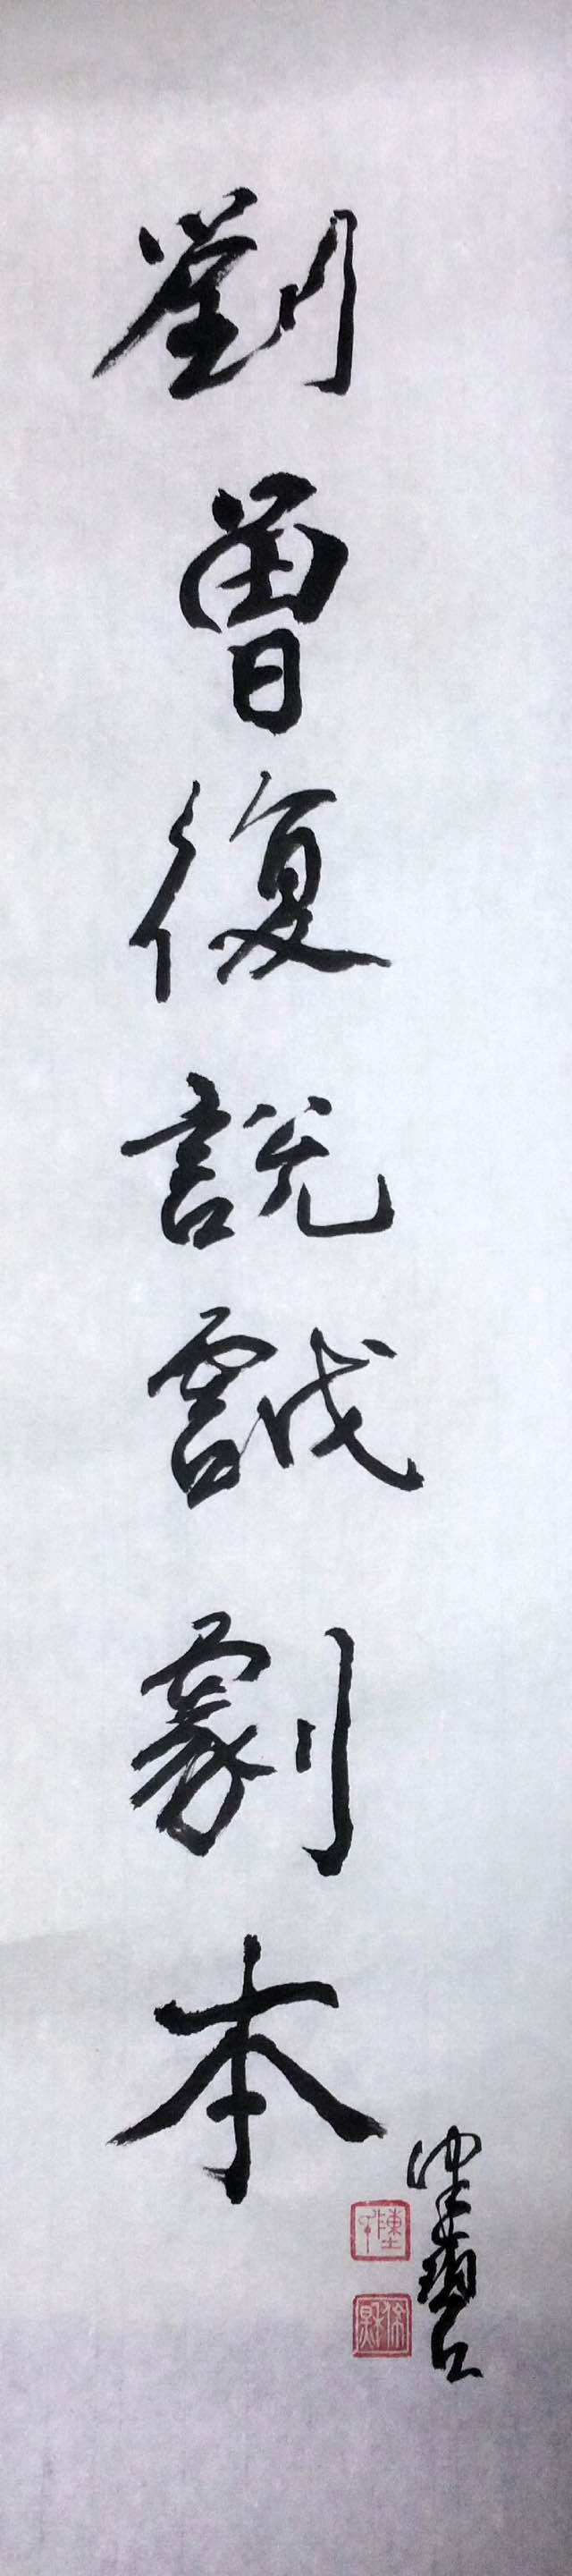
\includegraphics[height=1.30\textwidth,width=0.25\textwidth,viewport=0 0 620 2850,clip]{Figures_Peking-Opera/Liu_script-Inscription.JPG}
%\caption*{\hei 陈佩秋(谢稚柳~夫人)先生~题签}
\label{Chen-Peking_Opera_Script-Inscription-2015}
\end{figure}

\newpage
\pagestyle{empty}    % 清空页码                                      %
\begin{figure}[h!]
\centering
\vspace{+0.2in}
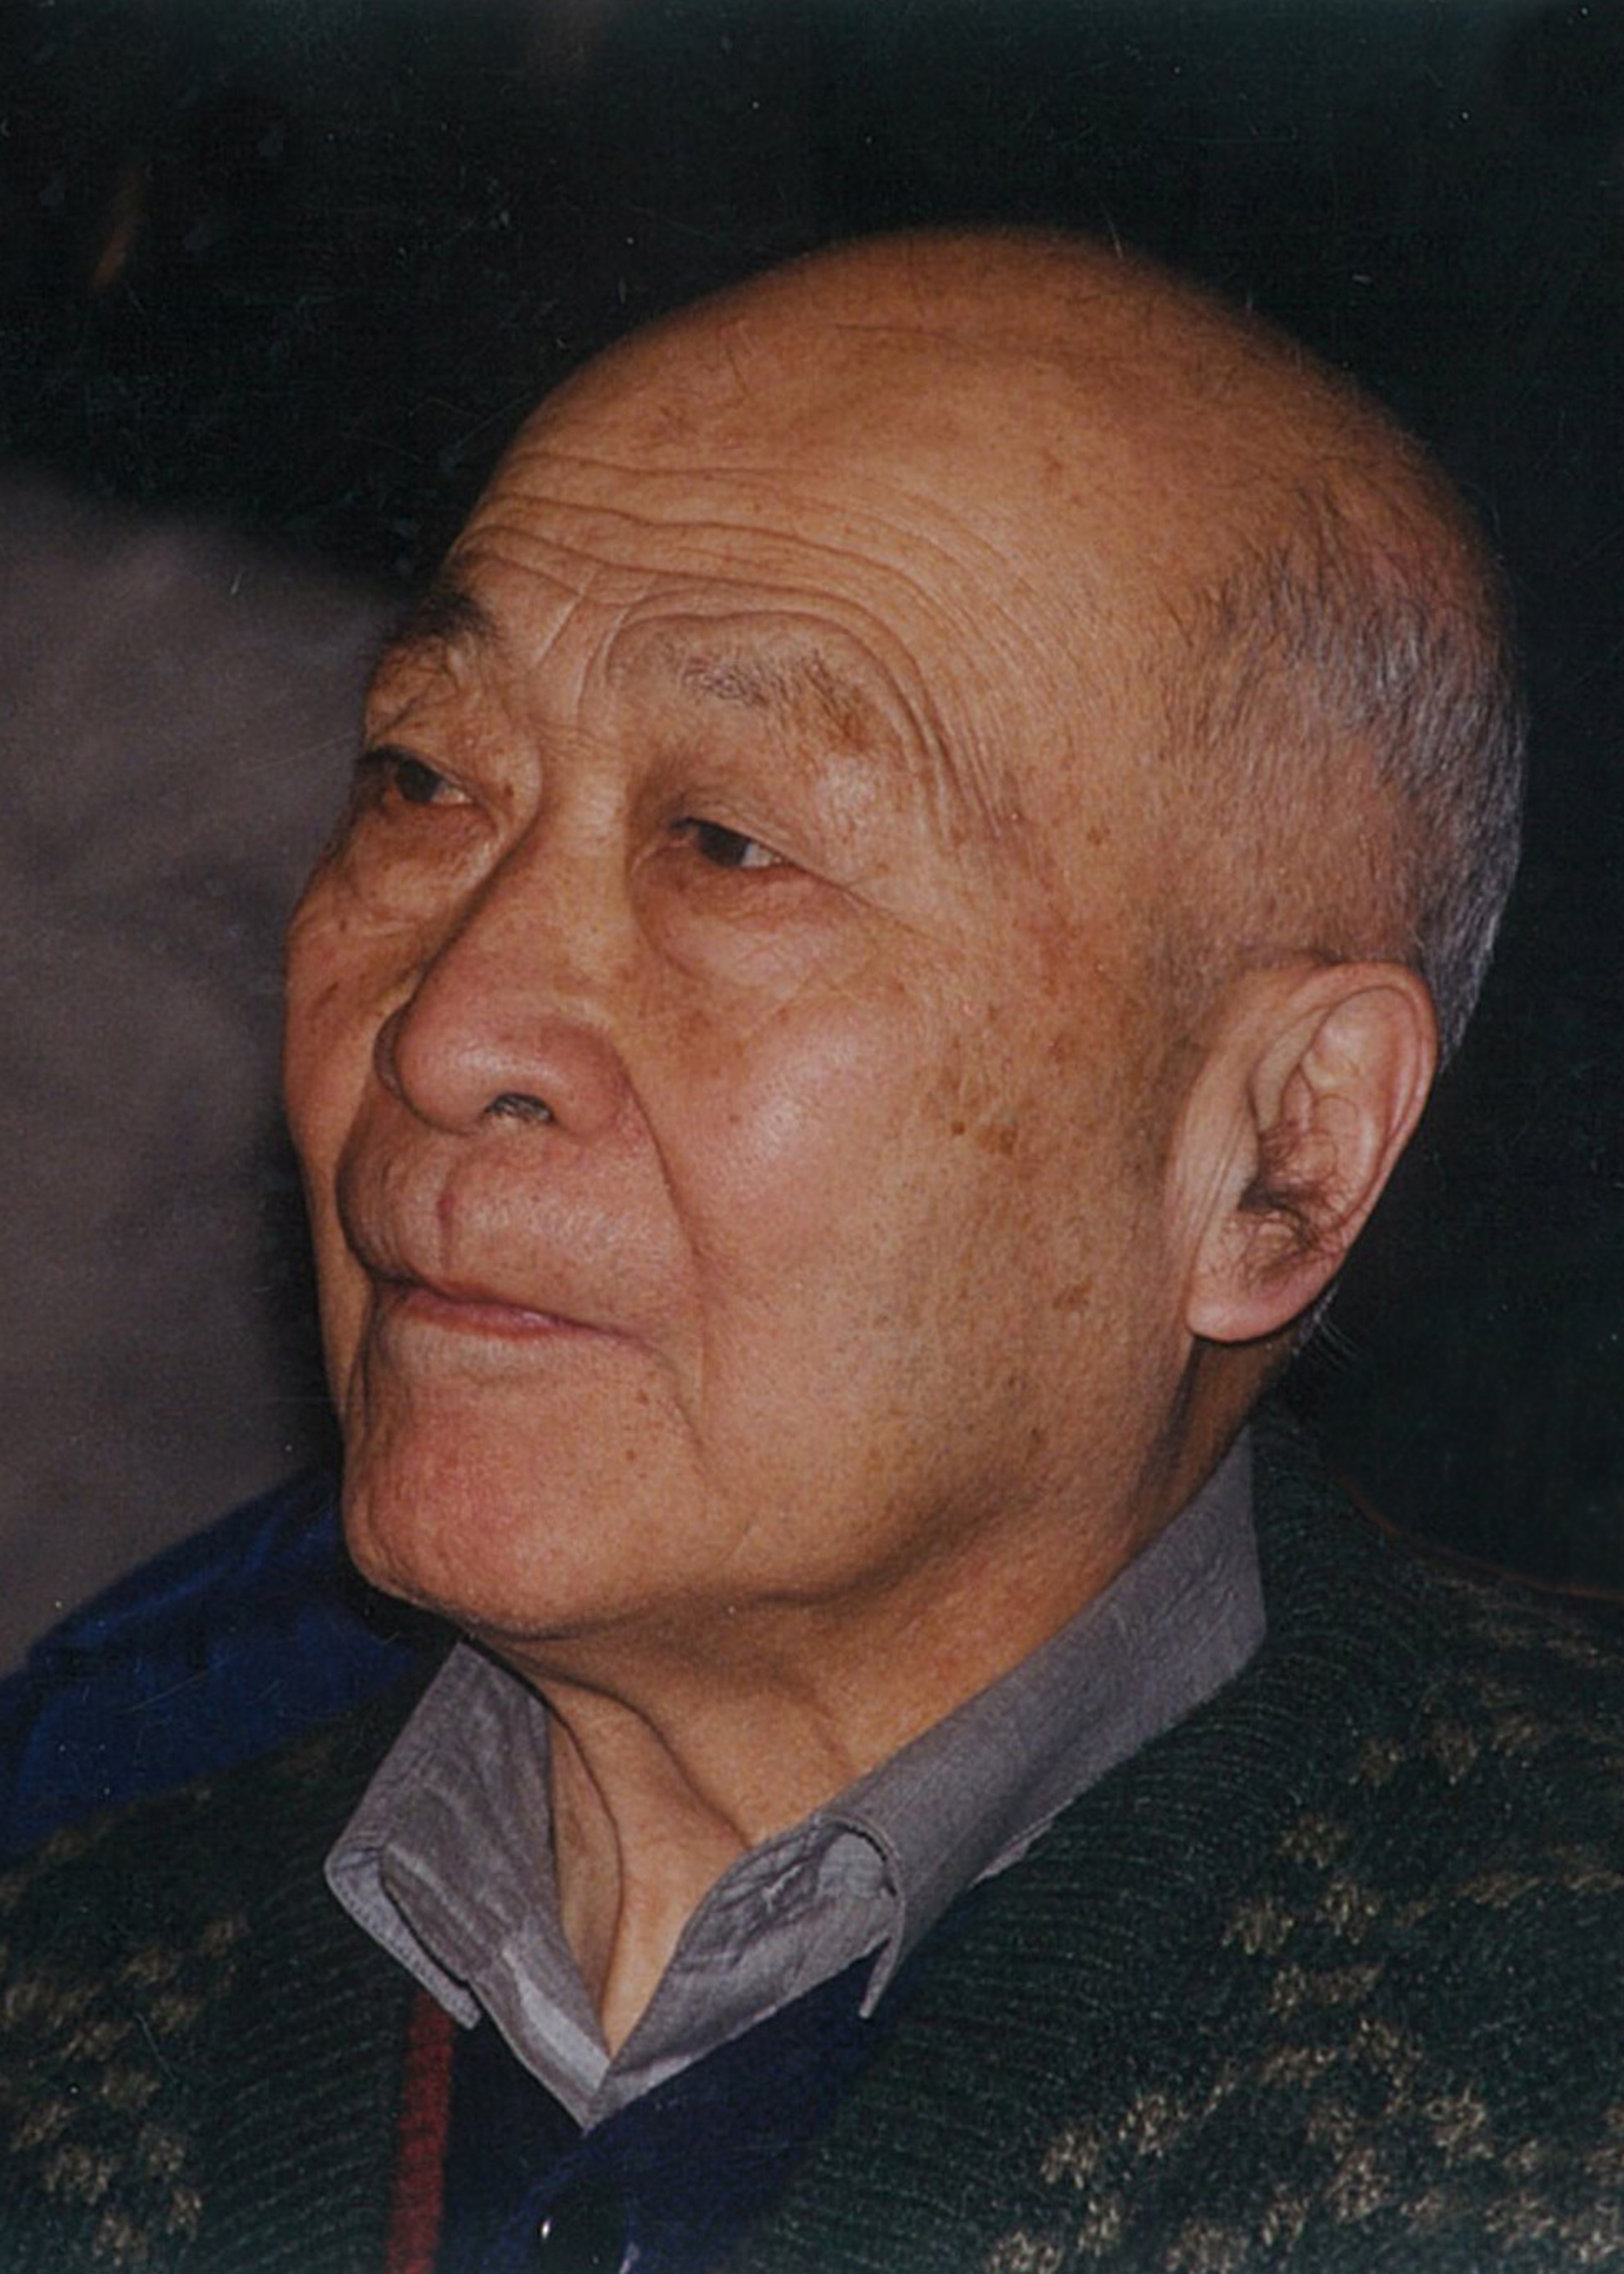
\includegraphics[height=1.20\textwidth,width=0.82\textwidth,viewport=0 0 360 520,clip]{Liu_Zengfu.jpg}
\caption*{\hei 刘曾复~教授~~(1914.11.9-2012.6.27)}
\label{Liu_Zengfu}
\end{figure}

\newpage
\begin{figure}[h!]
\centering
\vspace{-0.2in}
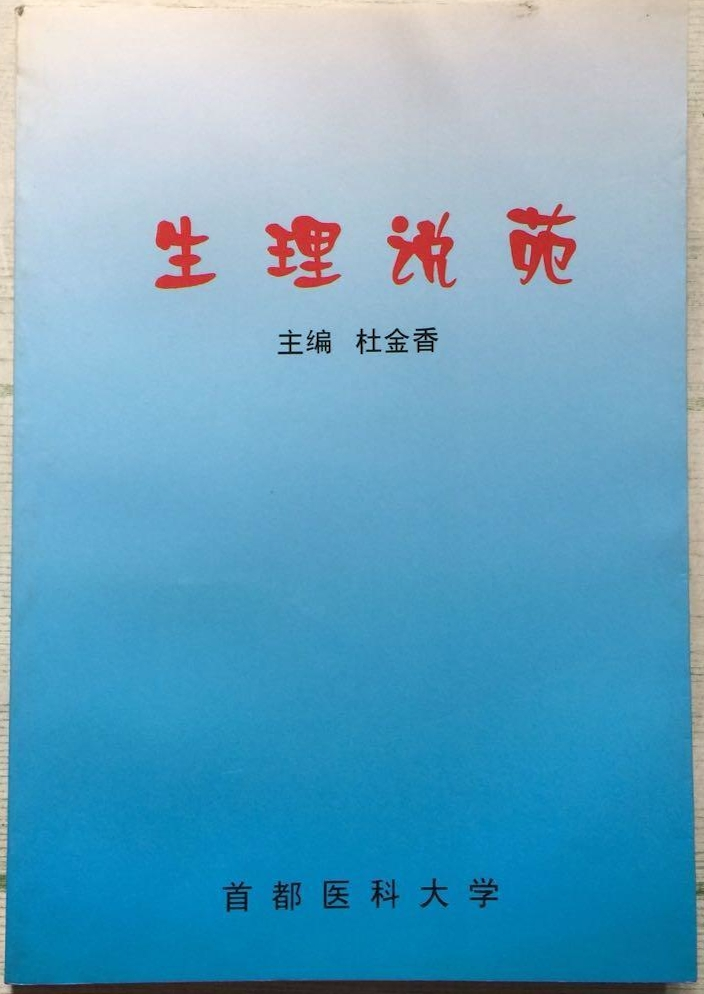
\includegraphics[height=0.65\textwidth,width=0.48\textwidth,viewport=0 0 700 1000,clip]{Liu-Physiology.jpg}
\label{Liu-Physiology}
\end{figure}
\begin{figure}[hbtp!]
\hspace*{-0.4in}
\begin{minipage}[t]{0.48\textwidth}
	\centering
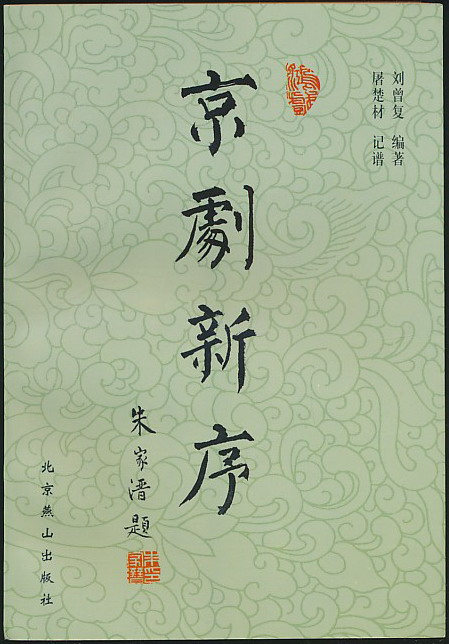
\includegraphics[height=1.50\textwidth,width=1.05\textwidth,viewport=0 0 450 650,clip]{Liu-Xinxu.jpg}
\end{minipage}
\hspace{0.3in}
\begin{minipage}[t]{0.48\textwidth}
	\centering
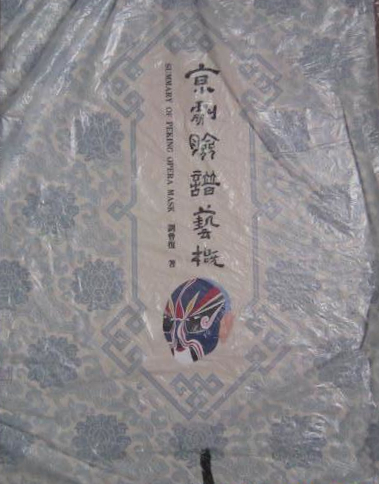
\includegraphics[height=1.50\textwidth,width=1.25\textwidth,viewport=0 0 410 490,clip]{Liu-Mask.jpg}
\end{minipage}
\vspace{1.0pt}
\caption*{\hei 刘曾复~教授~主要代表著作}
\label{Major_Works}
\end{figure}

\newpage
\begin{figure}[h!]
\centering
%\vspace{+0.2in}
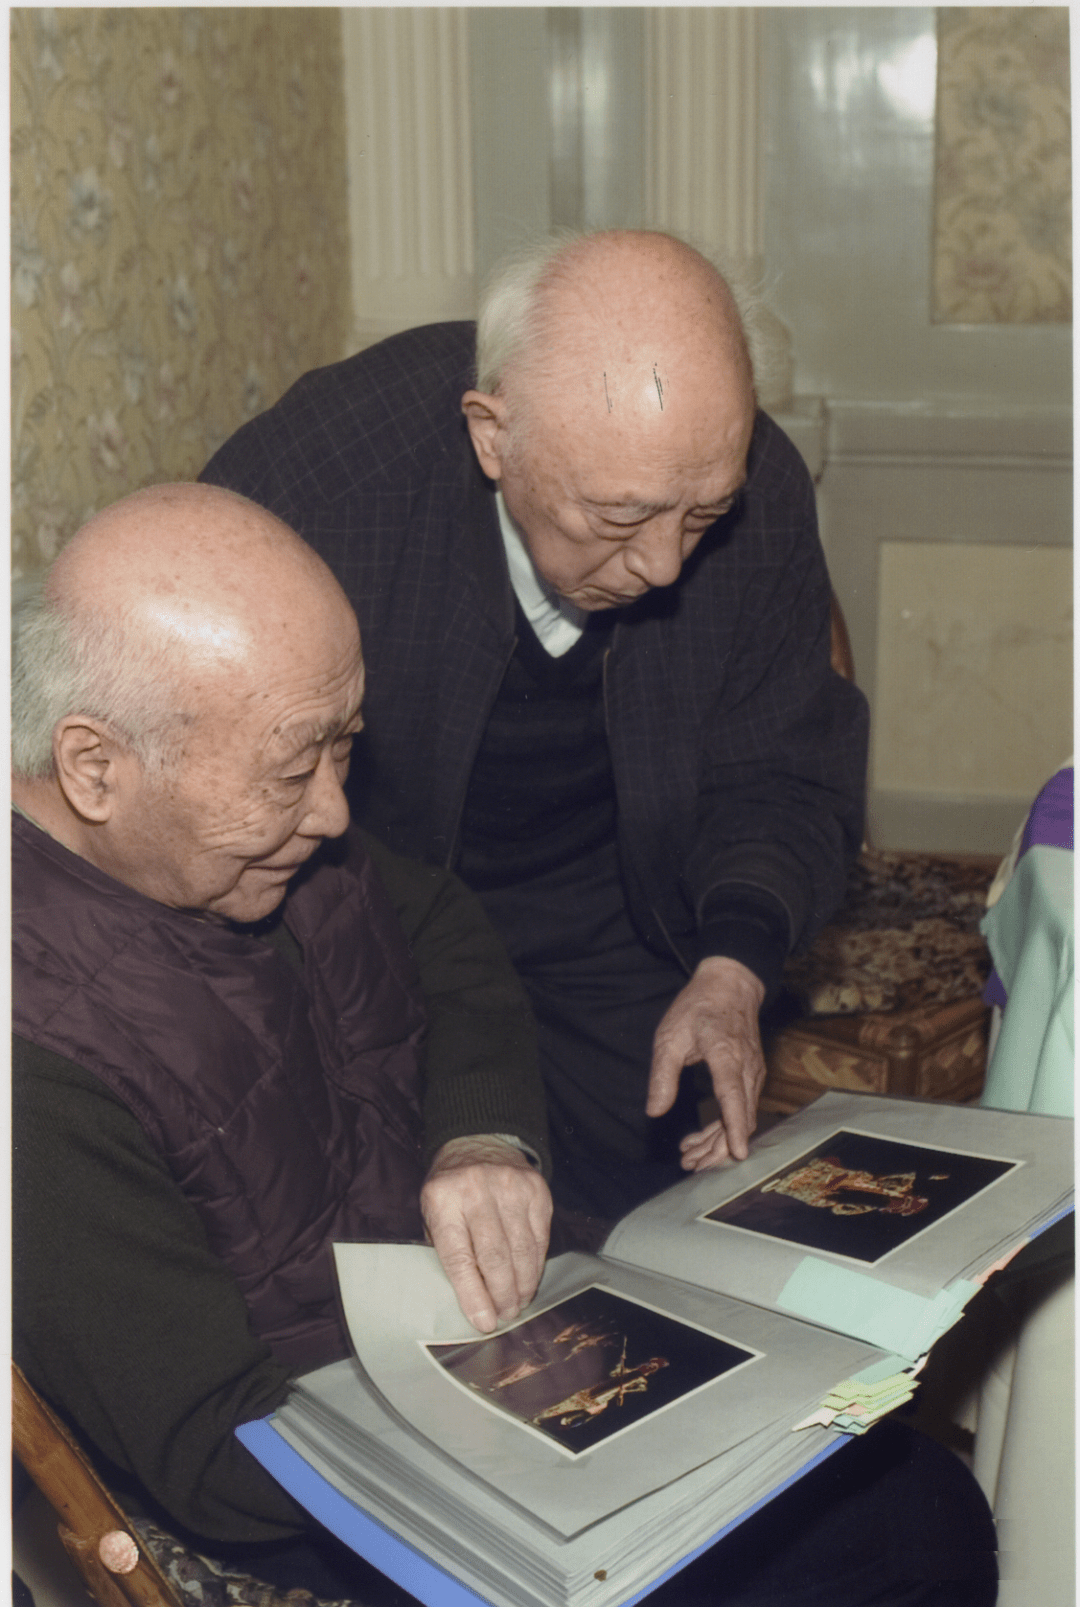
\includegraphics[height=1.38\textwidth,width=1.0\textwidth,viewport=0 0 1050 1550,clip]{Liu-Wu.png}
\caption*{\hei 刘曾复~先生~和~吴小如~先生}
\label{Collect_Liu_Wu}
\end{figure}

\newpage
\begin{figure}[h!]
\centering
%\vspace{-10.5pt}
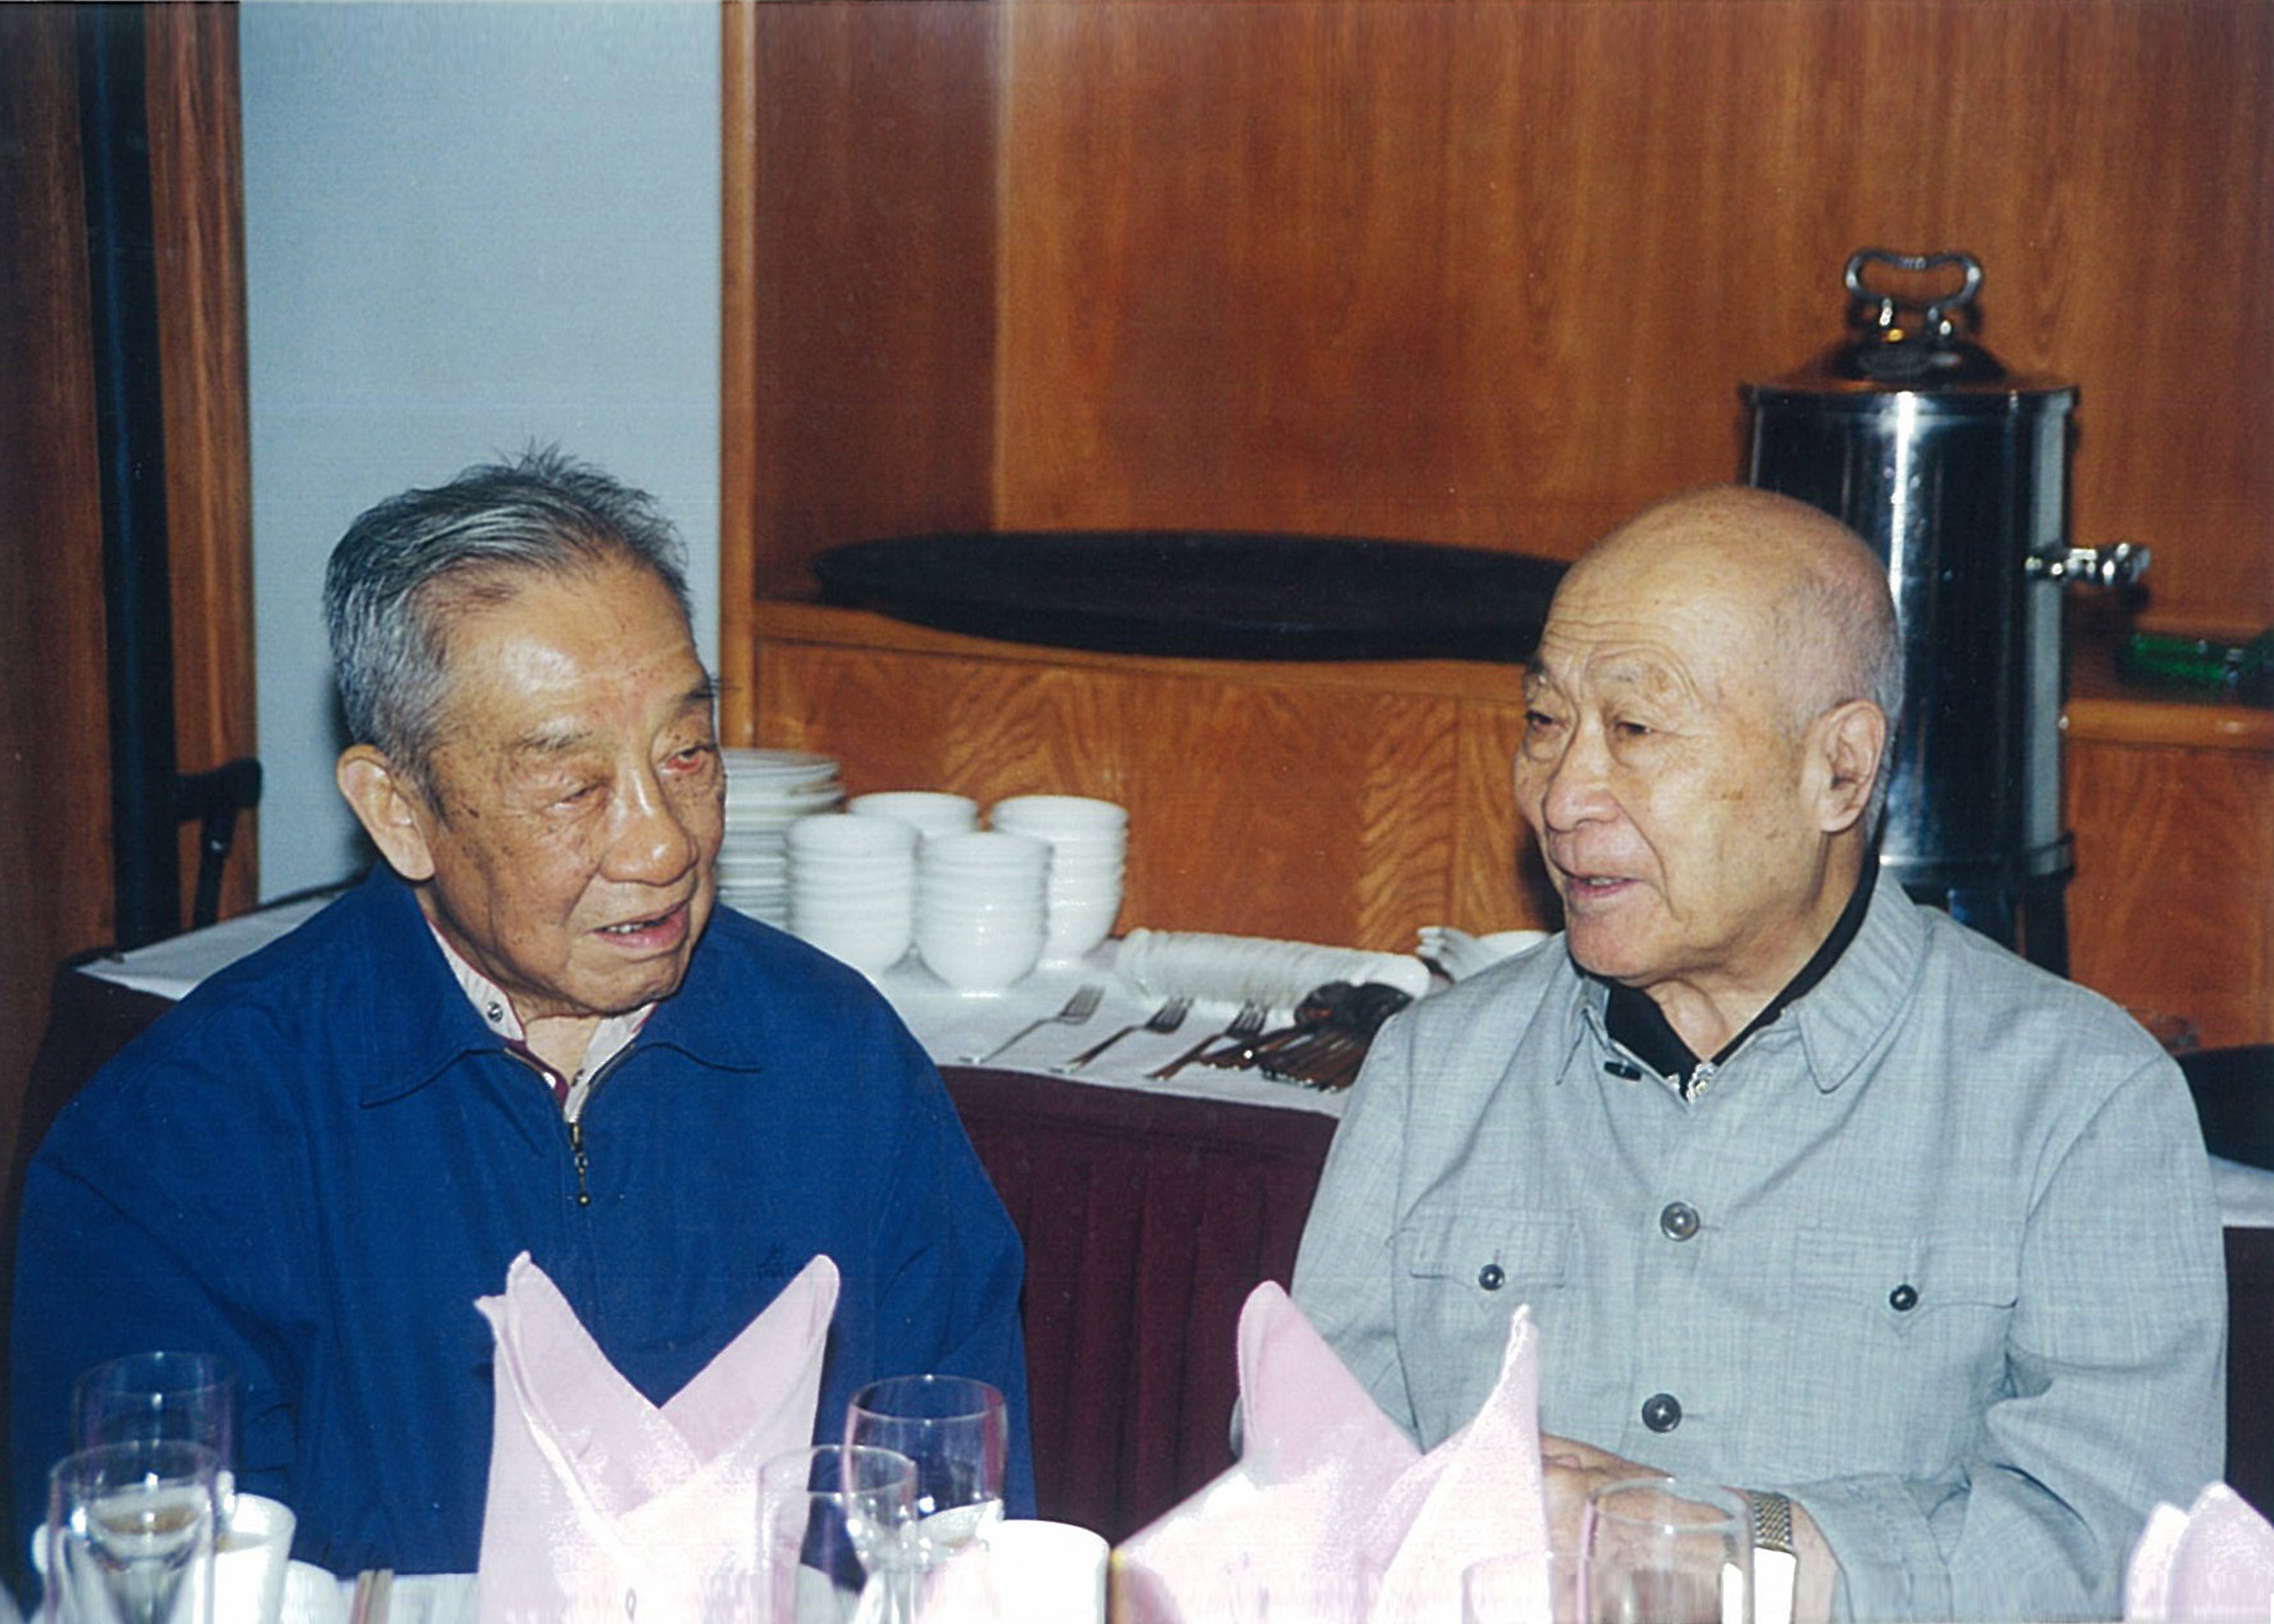
\includegraphics[height=0.60\textwidth,width=1.0\textwidth,viewport=0 0 500 300,clip]{Zhu-Liu.jpg}
\caption*{\hei 朱家溍~先生~和~刘曾复~先生}
\label{Collect_Zhu_Wu}
\end{figure}

\begin{figure}[h!]
\centering
%\vspace{-10.5pt}
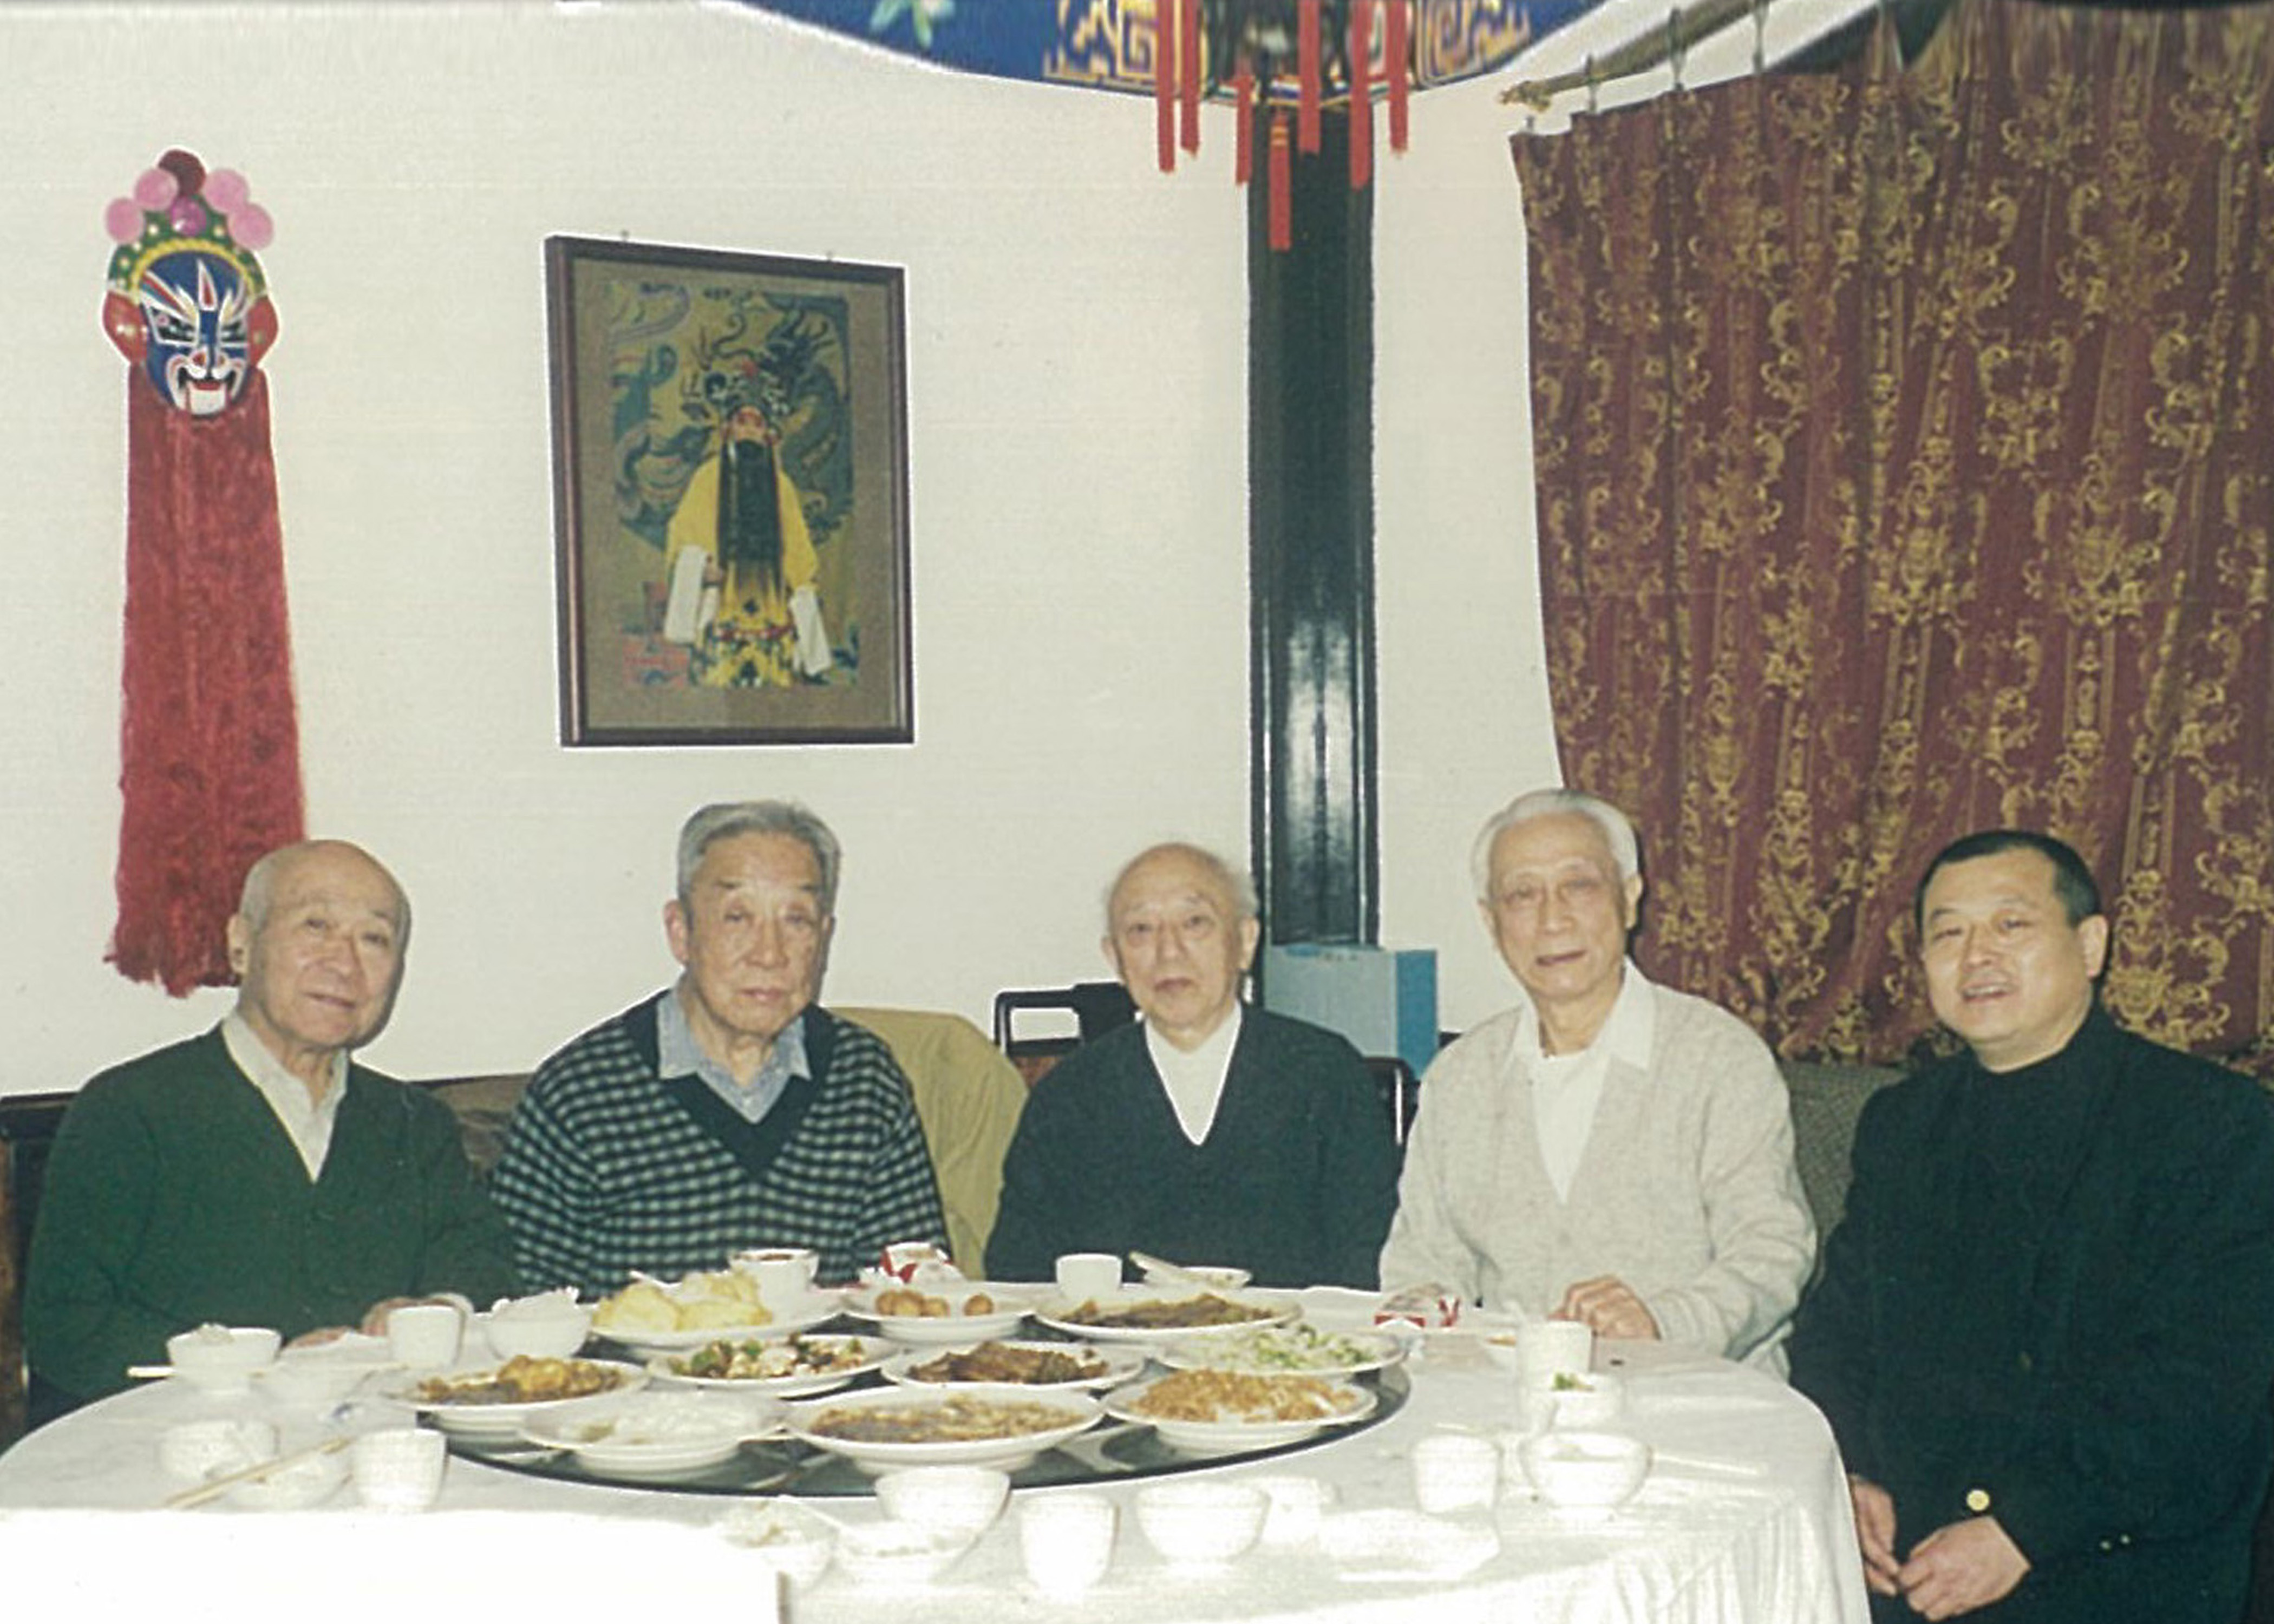
\includegraphics[height=0.60\textwidth,width=1.0\textwidth,viewport=0 0 500 300,clip]{Collect_Zhu-Liu-Wu-Wang.jpg}
\caption*{\hei 左起:~刘曾复~先生、朱家溍~先生、吴小如~先生、王金璐~先生~等~合影}
\label{Collect_Liy_Zhu_Wu_Wang}
\end{figure}

\newpage
\begin{figure}[h!]
\centering
\vspace{-0.6in}
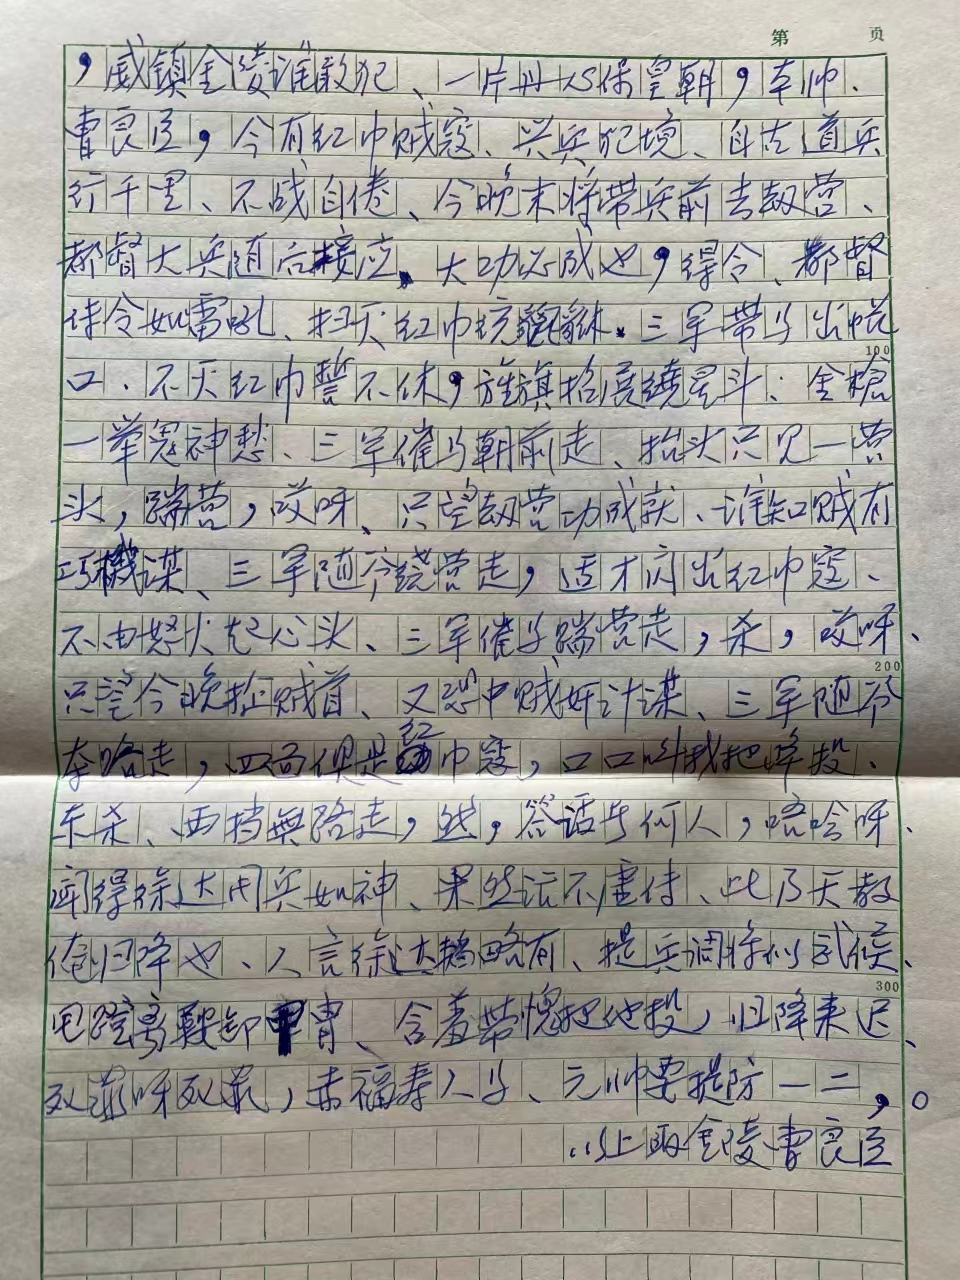
\includegraphics[height=0.68\textwidth,width=0.50\textwidth,viewport=0 0 950 1300,clip]{PekOpe_Liu-1.jpg}
\caption*{\hei 刘曾复~先生~抄录的《取金陵》曹良臣的单词}
\label{Liu-Script}
\end{figure}
\vspace{30pt}
\begin{figure}[hbtp!]
\hspace*{-0.5in}
\begin{minipage}[t]{0.53\textwidth}
	\centering
	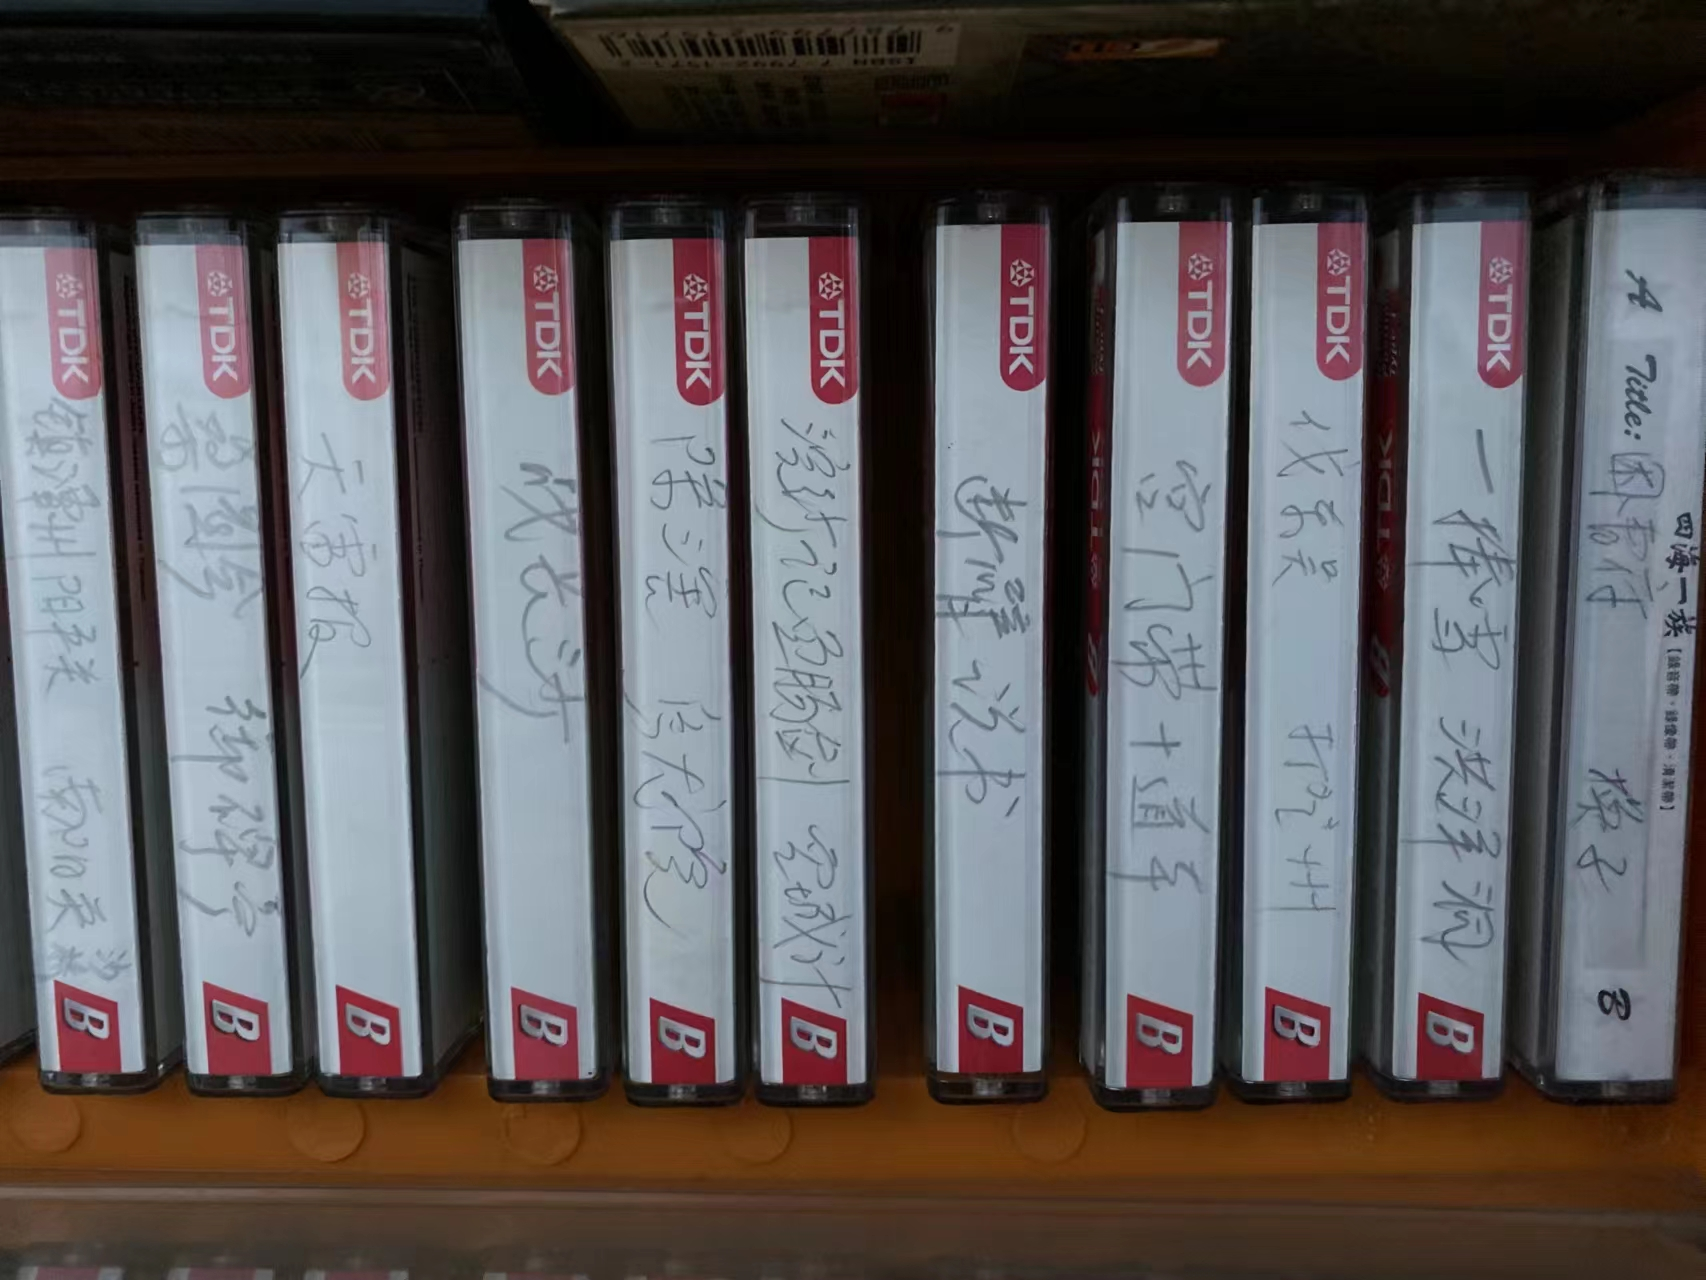
\includegraphics[height=1.00\textwidth,width=1.20\textwidth,viewport=0 0 1750 1300,clip]{PekOpe_Liu-2.jpg}
	\caption*{\hei \fontsize{8.5pt}{4.0pt}\selectfont{左:~刘曾复~先生~保存的部分说戏录音磁带}}
\end{minipage}
\hspace{0.6in}
\begin{minipage}[t]{0.43\textwidth}
	\centering
	\vspace{-3.7in}
	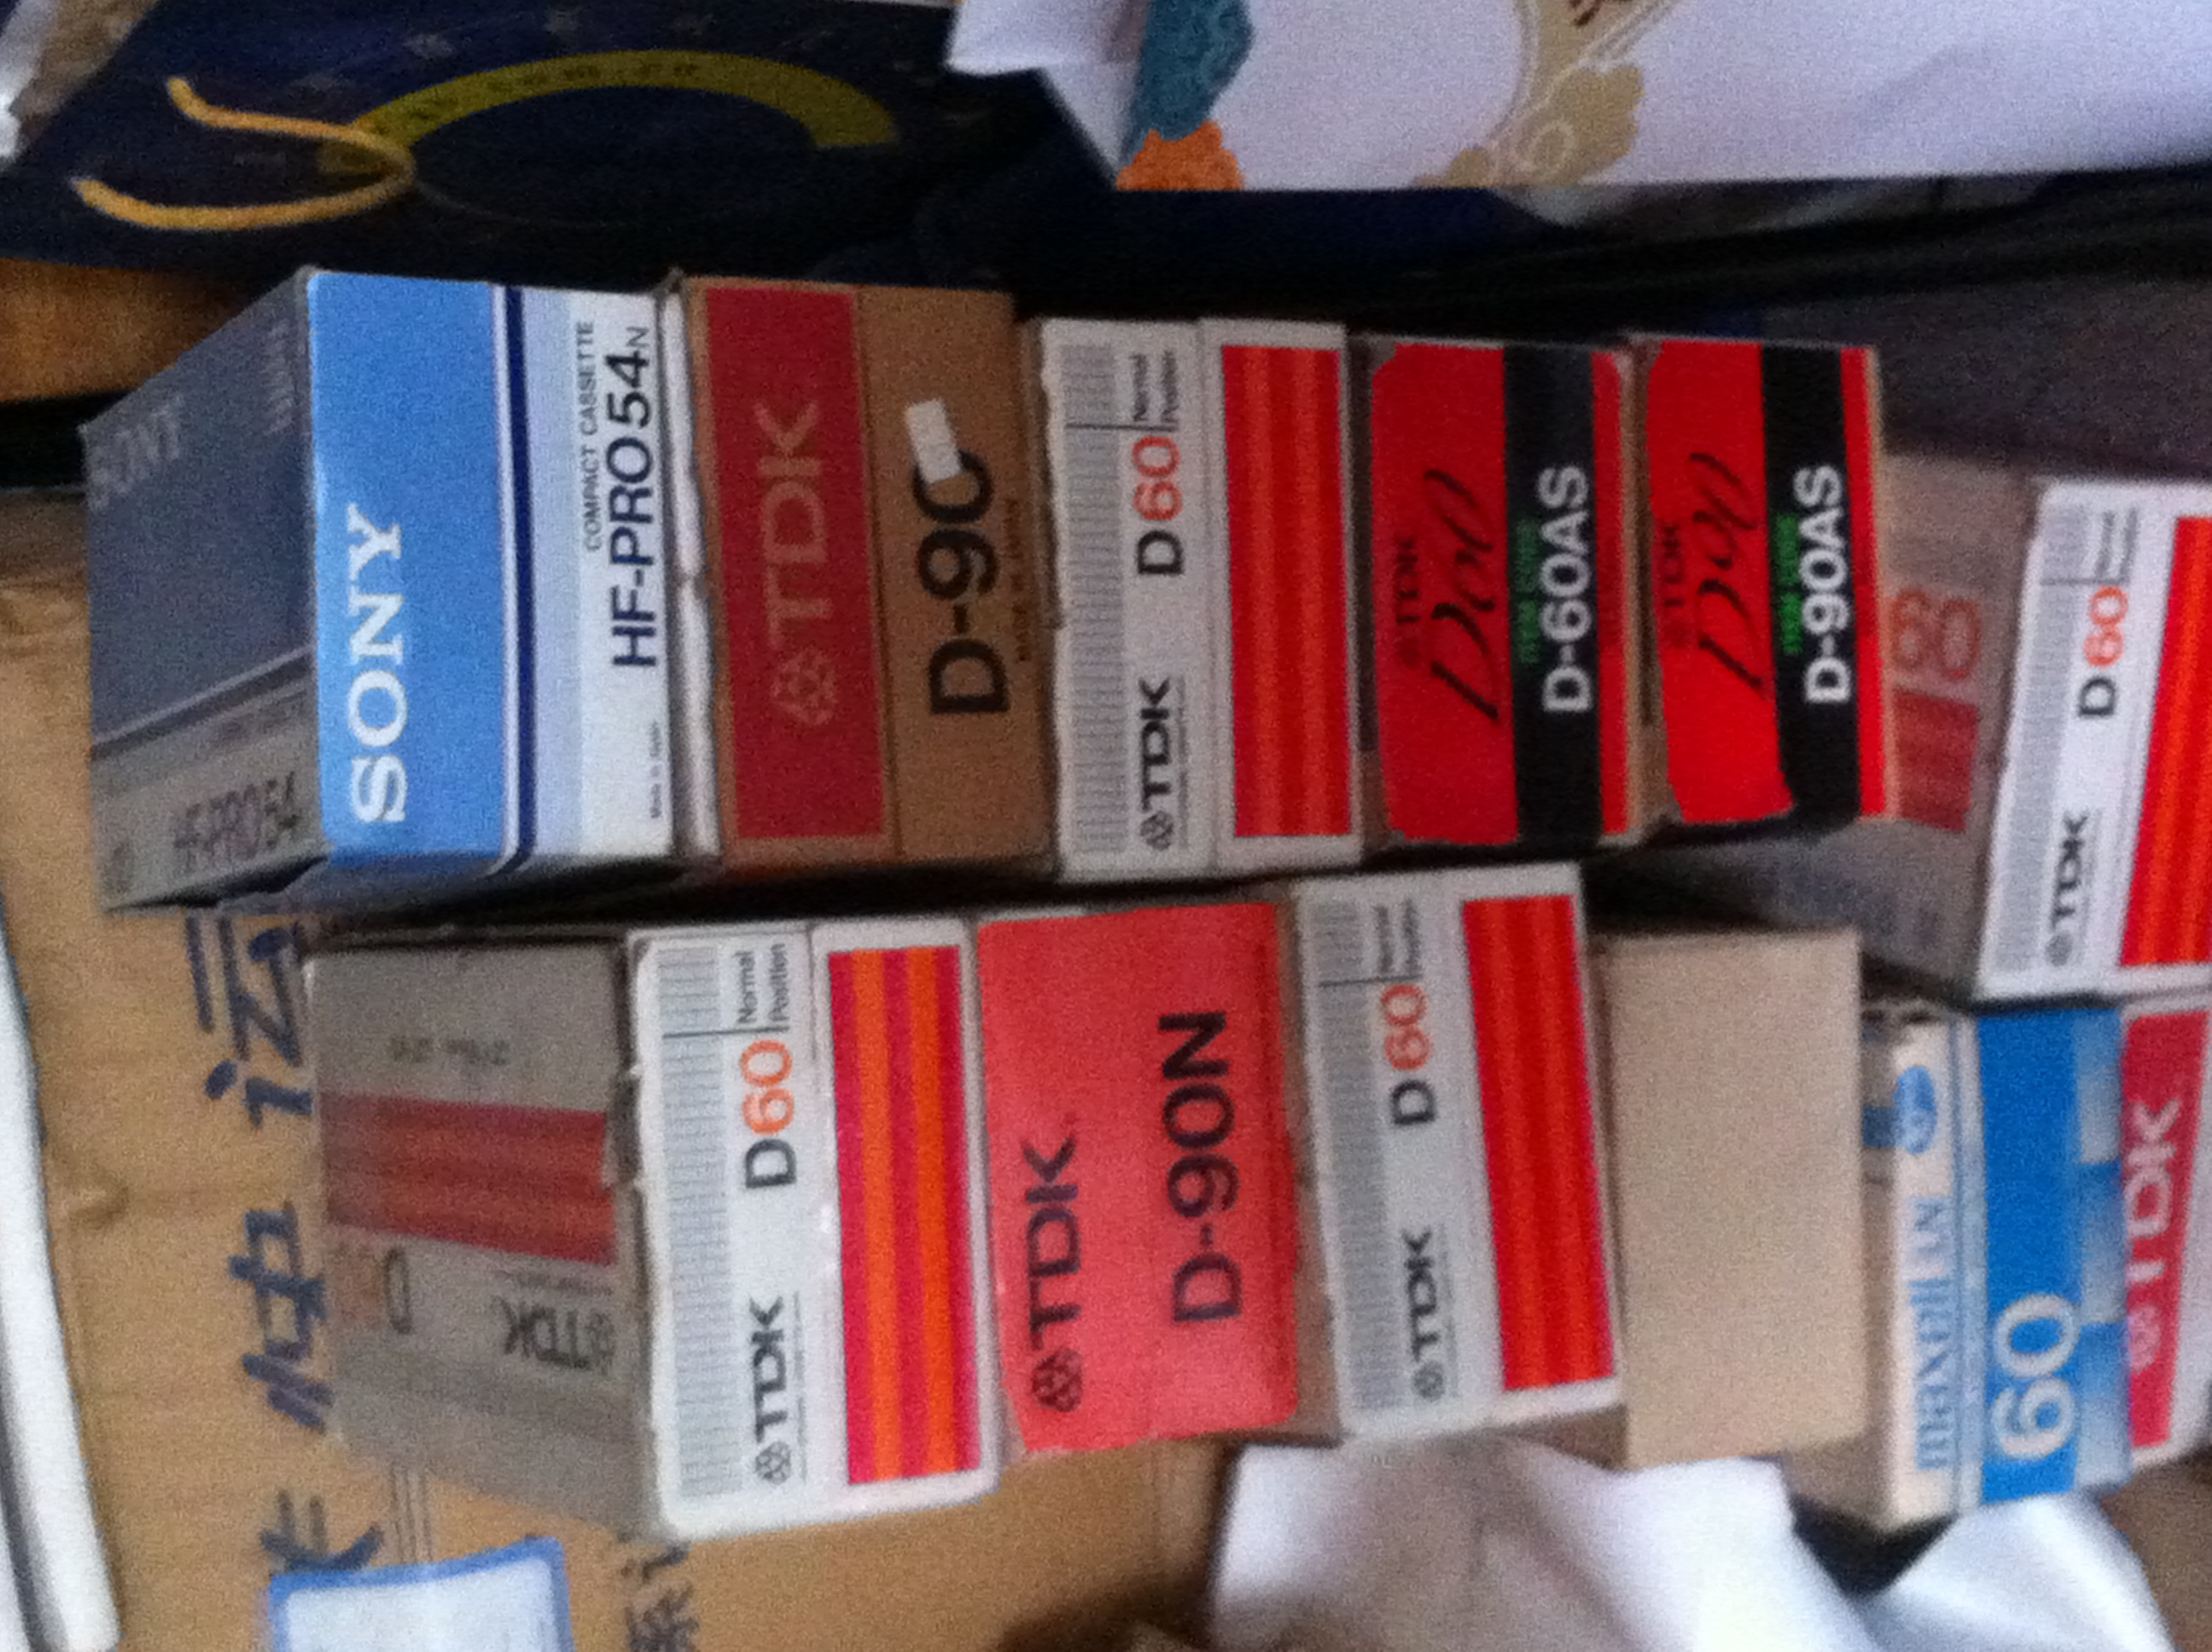
\includegraphics[height=1.10\textwidth,width=1.70\textwidth,angle=270, viewport=0 0 2750 1950,clip]{PekOpe_Wu-5.jpg}
%	\caption*{\hei \fontsize{8.5pt}{4.0pt}\selectfont{右:吴小如~先生~保存的刘曾复先生的说戏录音磁带}}
	\caption*{\hei \fontsize{8.5pt}{4.0pt}\selectfont{右:吴小如~先生~保存的各类说戏录音磁带}}
\end{minipage}
\label{Records}
\end{figure}
\newpage
\begin{figure}[h!]
\centering
\vspace{-0.6in}
	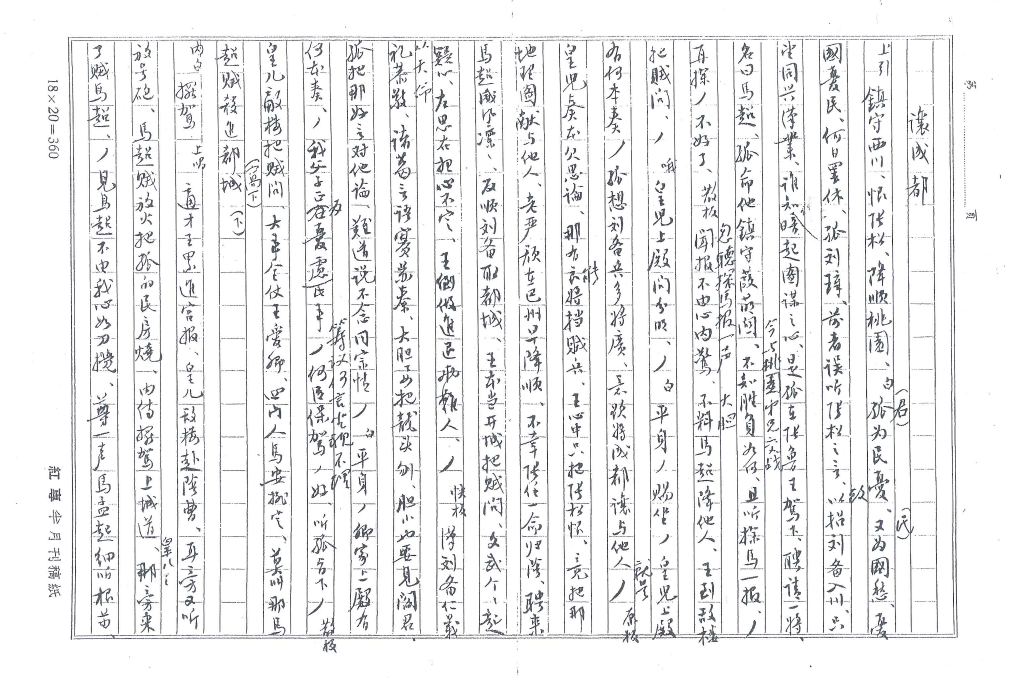
\includegraphics[height=0.50\textwidth,width=0.78\textwidth,viewport=0 0 750 470,clip]{PekOpe_Wu-script-1.png}
	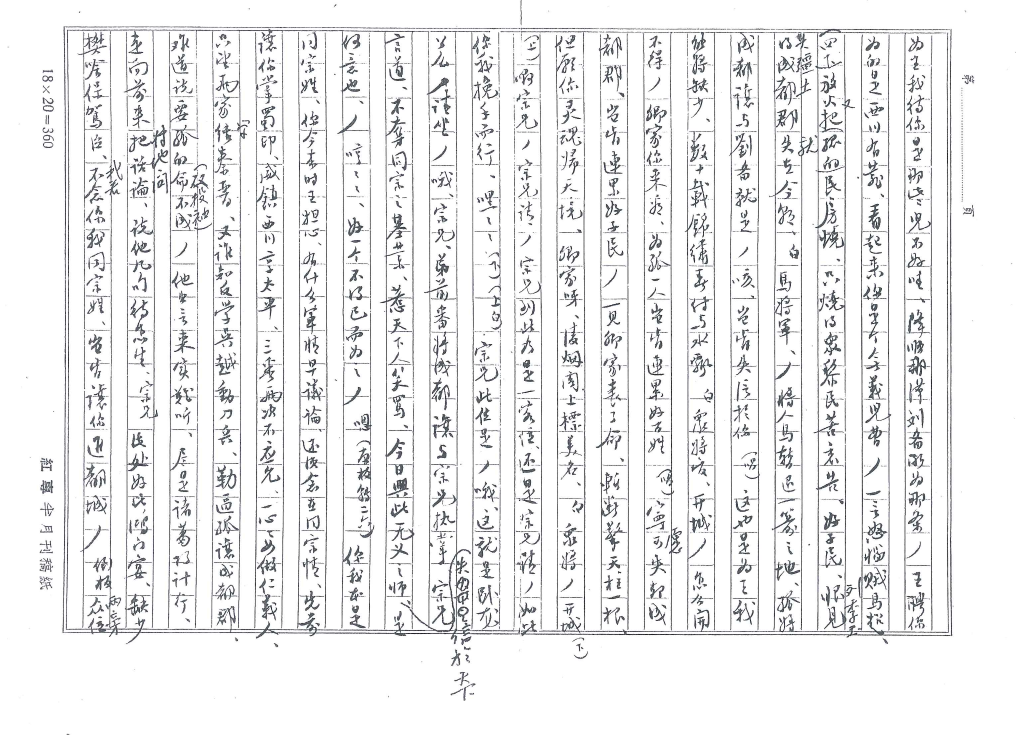
\includegraphics[height=0.50\textwidth,width=0.81\textwidth,viewport=0 0 750 520,clip]{PekOpe_Wu-script-2.png}
	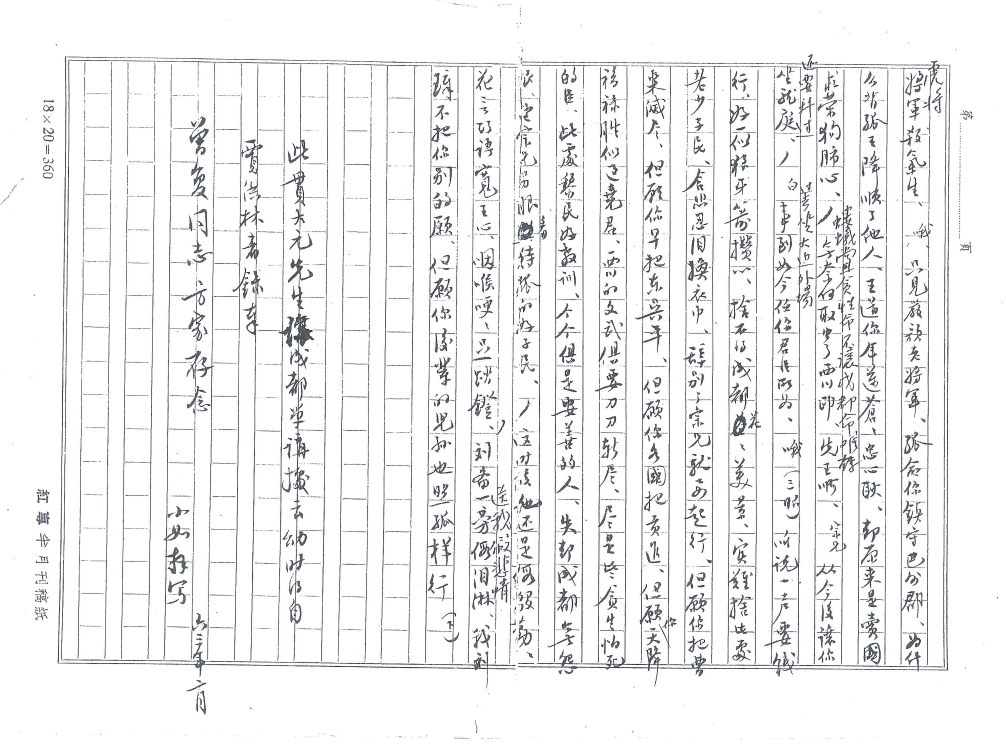
\includegraphics[height=0.50\textwidth,width=0.8\textwidth,viewport=0 0 750 500,clip]{PekOpe_Wu-script-3.png}
%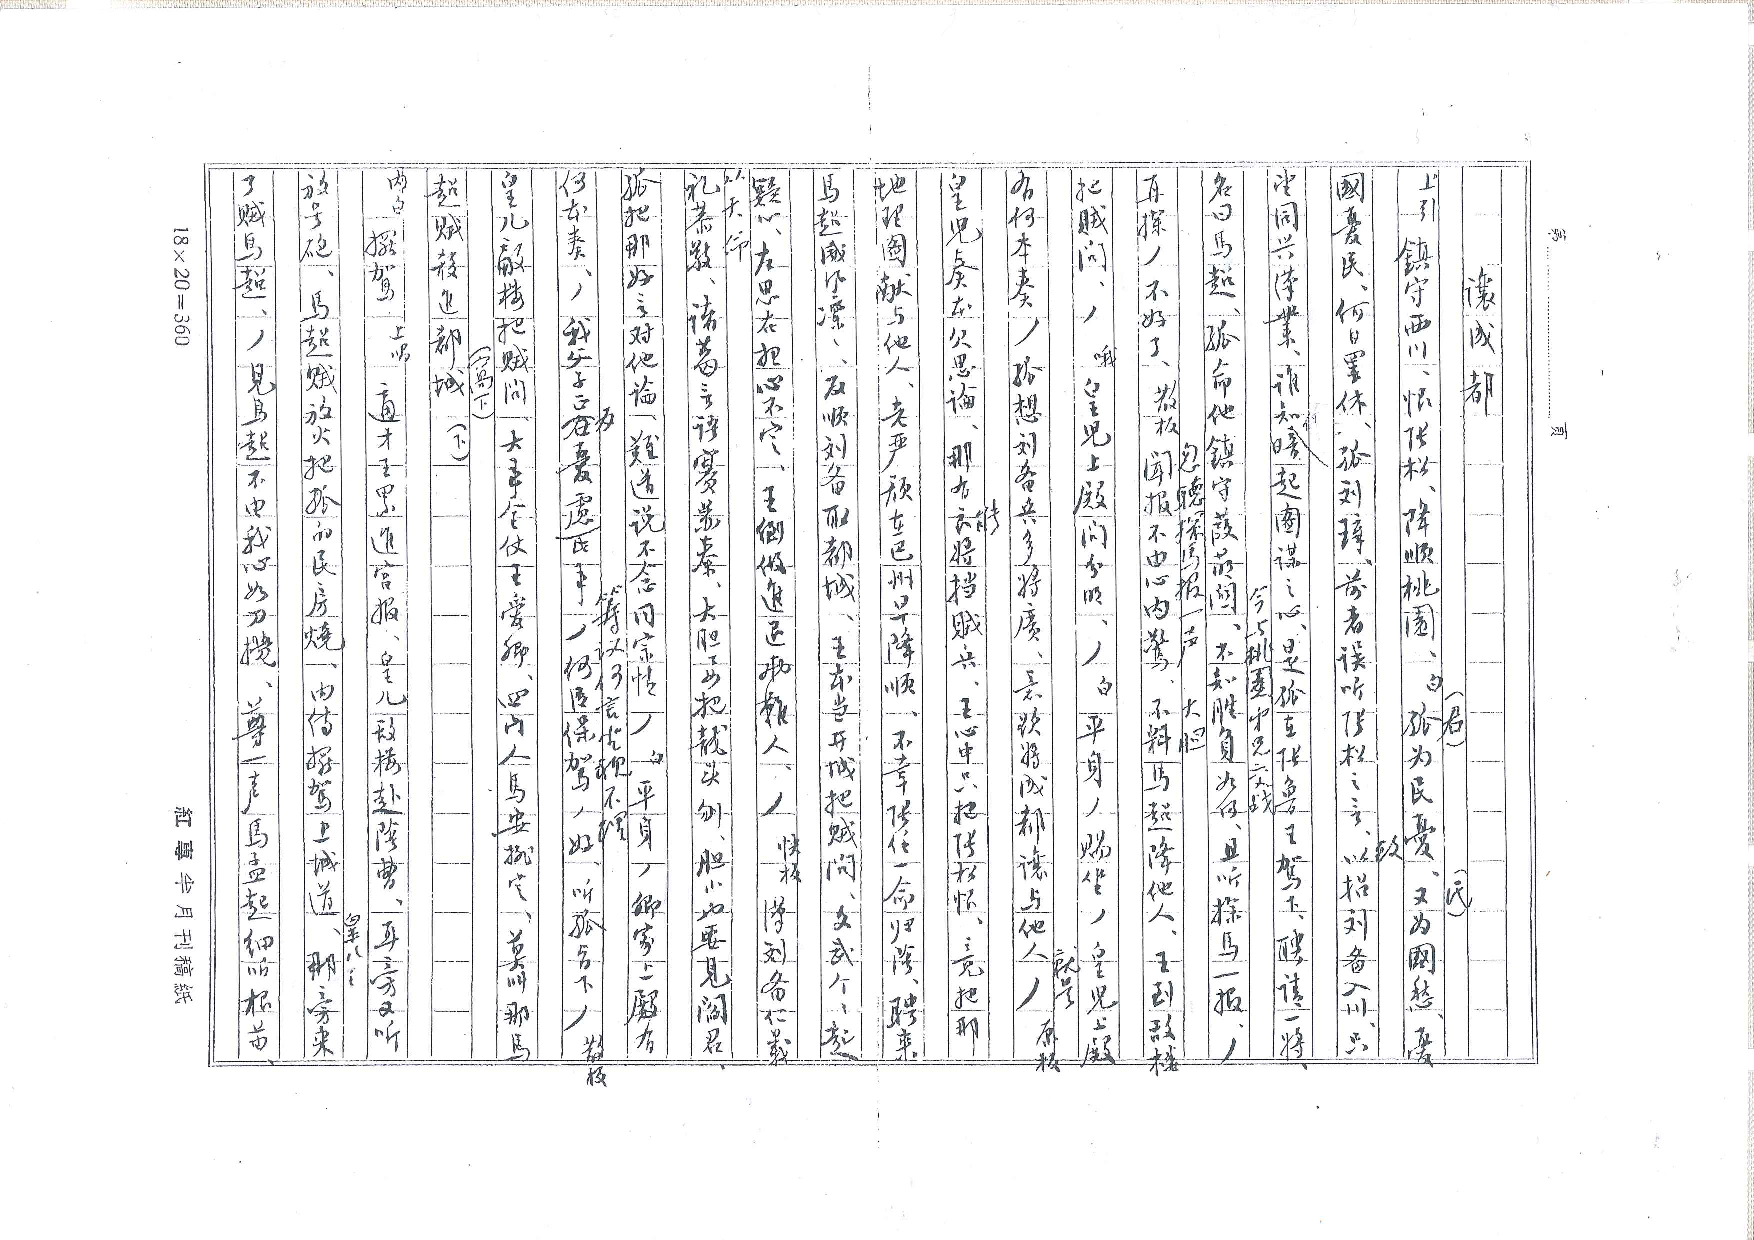
\includepdf[fitpaper]{PekOpe_Wu-script.pdf}
\caption*{\hei 吴小如~先生~抄录的~《让成都》刘璋的单词(贯大元~先生~传)复印件,刘曾复~先生~作了修改}
\label{Wu-Script}
\end{figure}

\newpage
\begin{figure}[h!]
\centering
%\vspace{-10.5pt}
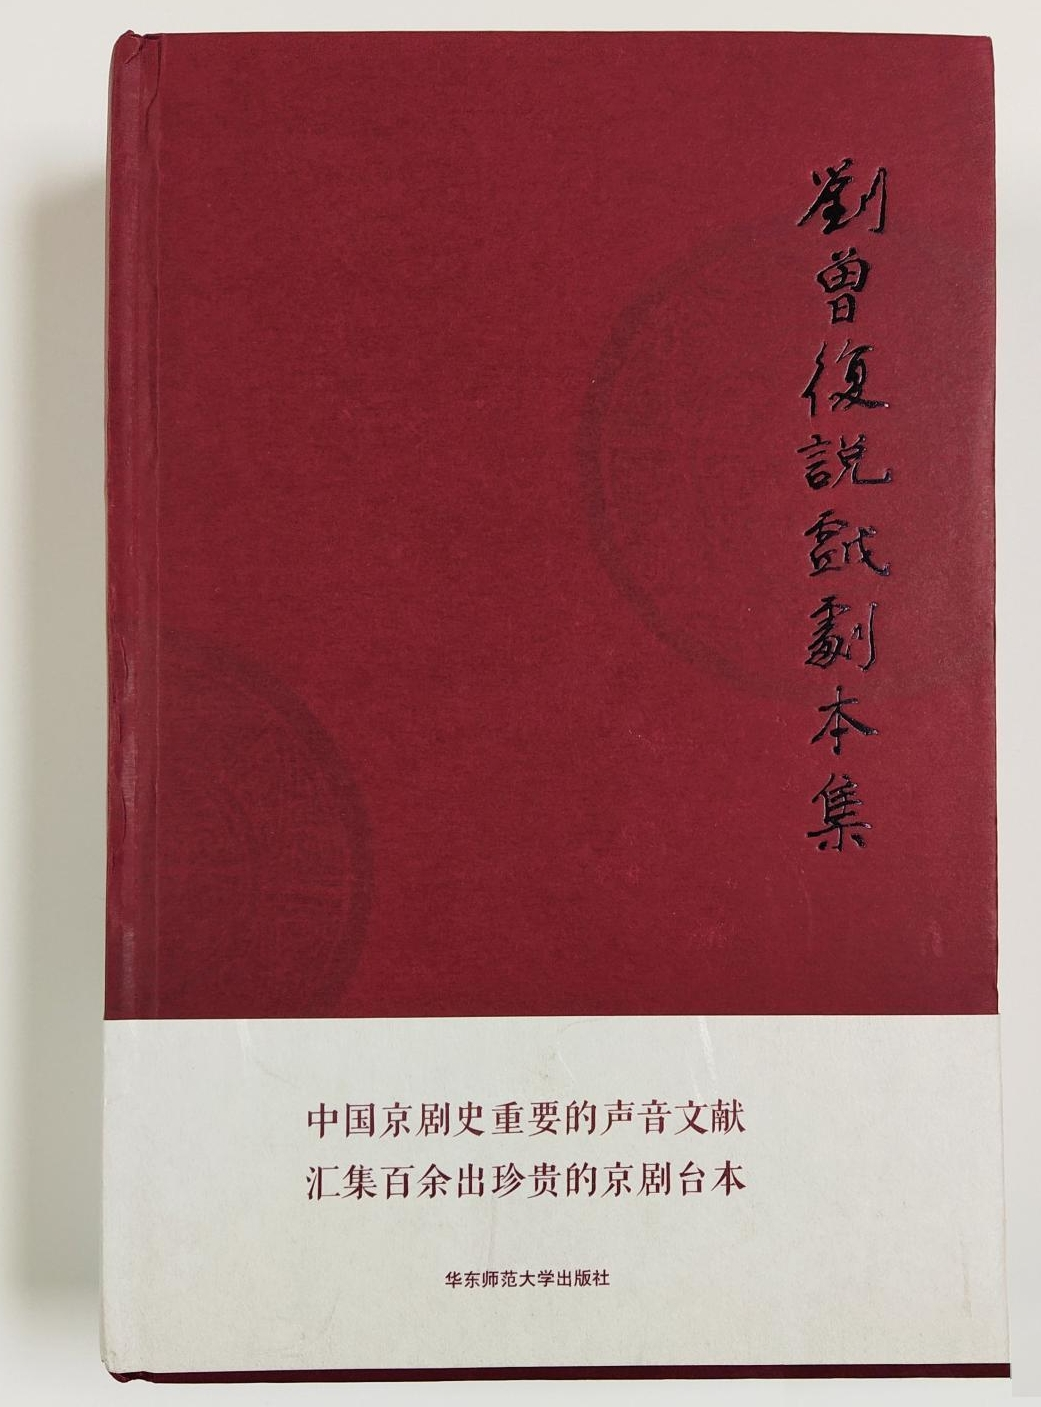
\includegraphics[height=1.30\textwidth,width=1.02\textwidth,viewport=0 0 1030 1400,clip]{Figures_Peking-Opera/Liu_script.jpg}
\caption*{\hei \fontsize{8.5pt}{4.0pt}\selectfont{《刘曾复说戏剧本集》初版~(上海~华东师范大学出版社~2015.08)~书影}}
\label{Peking_Opera_Script}
\end{figure}
%\keywords{Keyword1; Keyword2; Keyword3}


%%\newpage
\newpage
\phantomsection %实现目录的正确跳转
\setcounter{page}{0}
\pagenumbering{roman}
%\hypertarget{ux8bf4-ux660e}{
\addcontentsline{toc}{section}{\hei 说~~~~~~明}
	\section*{\hei \large 说\hspace{35pt}明}\label{ux8bf4-ux660e}%}
\pagestyle{fancy}    %与文献引用超链接style有冲突
\chead{说~明} % 页眉中间位置内容

\setlength{\parindent}{24pt}{     %
	此为个人整理的刘曾复教授说戏录音的文本稿,\textbf{主要根据刘曾复先生为中国戏曲学院提供的百余出说戏录音为底本,并结合刘曾老在其余场合的说戏录音}\upcite{Liu-Shuoxi-Record}%\textsuperscript{{[}1{]}}
\textbf{整理完成的}。其中《太平桥》、《盗宗卷》、《梅龙镇》、《辕门斩子》、《摘缨会》、《上天台》、《一捧雪》、《卖马》、《南阳关》的``总讲本''主要依据《京剧新序》\upcite{Liu_Xinxu-I,Liu_Xinxu-II}%\textsuperscript{{[}2{]}.}
中收录的刘曾复先生整理的剧本并结合说戏录音整理完成;《马鞍山》、《战长沙》的``总讲本''则参考了李舒先生遗作《涉艺所得》\upcite{Li-SheyiSuode}%\textsuperscript{{[}3{]}.}
收录的刘曾复先生手书稿和传本并结合说戏录音整理完成的。\textbf{有关剧目中的把子,主要摘录自}《京剧新序》和《京剧老生把子见闻录》\upcite{XQYS1-32_1983}%\textsuperscript{{[}4{]}.}
一文记录的开打和舞台调度。

除了上述《太平桥》等十一出剧目,其余剧目的场次安排主要参考了《京剧汇编~(1-109集)》\upcite{Jingju-Huibian-1}%\textsuperscript{{[}5{]}.}
、《传统剧目汇编》\upcite{Jingju-Huibian-2}%\textsuperscript{{[}6{]}.}
、《京剧丛刊~(1-50集)》\upcite{Jingju-Congkan}%\textsuperscript{{[}7{]}.}
、《清车王府藏曲本(全印本)》\upcite{CWFCQB}
和``中国京剧戏考''网站\upcite{PekingOpera-Scripts}%\textsuperscript{{[}8{]}.}
上的相应的剧目的安排,个别剧目的词句也参考了,``中国京剧老唱片''网站\upcite{PekingOpera-OldRecords}%\textsuperscript{{[}9{]}.}
上载的老唱片戏词。

剧目按照剧中人物年代排列,部分剧目的年代排序参考了《京剧大戏考》\upcite{Chai-DaXikao}%\textsuperscript{{[}10{]}.}
和《京剧知识词典(增订版)》\upcite{PekingOpera-Dictionary}%\textsuperscript{{[}11{]}.}
中的剧目顺序。

\vskip 5pt
基于全面、客观、忠实的记录原则,整理剧目文字的标记说明如下:
\begin{enumerate}
\def\labelenumi{\arabic{enumi}.}
\item
	{\CJKfamily{hei}因为本人学识浅陋、加之录音带存年较久,因此文字中有不少存疑处。凡是存疑处,尽量用\textcolor{red}{红色字体}标出,}表明此处可能文辞欠通顺,或只是根据字音听写臆测的词句;
\item
	{\CJKfamily{hei}刘曾复先生腹笥渊博,在不同的场合说戏时,即使是同一出戏,个别词句也略有出入,文本中尽量作了标注:~}

\begin{enumerate}
\def\labelenumi{\arabic{enumi}.}
\item
  每个剧目中凡有出入的唱、念词句标注为:

\begin{quote}
	\underline{\textrm{XX}词1}~({\akai 或}:~\textrm{XX}词2;~\textrm{XX}词3;$\cdots{}\cdots${})
\end{quote}
\begin{quote}
	\underline{\textrm{XX}句1}~({\akai 或}:~\textrm{XX}句2~{\akai 或}:~\textrm{XX}句3;$\cdots{}\cdots${})
\end{quote}

\def\labelenumi{\arabic{enumi}.}
\setcounter{enumi}{1}
\item
  每个剧目中可不念或某些衬字的唱、念标注为:

\begin{quote}
	(\textrm{XX}词句)
\end{quote}
\end{enumerate}

\def\labelenumi{\arabic{enumi}.}
\setcounter{enumi}{2}
\item
  \textbf{除``总讲本''外,``单词本''中,与表演配合的其他人物唱、念(盖口)标记为}:
\begin{quote}
	(人物\hspace{30pt} 唱、念词句\textrm{XXX}。)
\end{quote}
\item
  \textbf{在本人的知识范围内,对一些生僻的典故、词汇作了简要的注解。}
\item
  \textbf{刘曾复先生对唱、念中的虚词(衬字、垫字或语气词)非常重视,但文本中仅对极少部分虚词用小字号字体作了标注,挂一漏万。唱、念中虚词的使用,建议读者以先生的录音为准。}
\item
  \textbf{由于文字记录的功能有限,此书辑录的主要是说戏的文字内容,关于舞台表演过程中的唱、念的明细要求,本文都没有标注。}
\end{enumerate}
}
%----------------------------------------------------------------------------------------------------------------------------------------------------%

%
\newpage
\renewcommand{\thefootnote}{\roman{footnote}}
\setcounter{footnote}{0}
\phantomsection %实现目录的正确跳转
\pagestyle{fancy}    %与文献引用超链接style有冲突
\chead{序} % 页眉中间位置内容

\centering{《京剧献征》序}

一事有一事之运数,其通也不可遏,其穷也不可挽。皮黄独不然耶?方其通也,虽人人言其穷,无益也。有言至谭鑫培而穷者,乃有流派之盛矣;~有言至梅、杨、余而穷者,乃有众美之备矣。方其穷也,虽人人言其通,无益也。言样板,言振兴,亦不可谓不有力,而终视其倾耳。

吾言若此,决有恨之者曰:``子非爱皮黄者,故忍为是言也。''岂知吾哉!吾惟惜其之倾也,故有是言尔。盖必知其事之运数,乃能集其事。方其穷也,斯有穷时之应,庶得其道。而反以通时之应,必南北其辕辙矣。

吾所以赏明人之词学者以此。盖当元之季,词为曲所夺,其穷也必。乃有二三子者,斤斤保此宋人之遗作,使不失坠。一逢其运会,竟得清人之再兴,遗惠正自不浅也。且夫宋人,固能填词矣,而未必能知词,必待清人而后知之。无明人保有之功,词学之亡,岂待言哉!

吾人之于皮黄也,亦明人之于词学尔。方其穷也,不汲汲续其将绝之运命,而斤斤保其已得之成绩,静观默存,待其运会。吾不敢必皮黄有再兴之日,后来能因是而知皮黄,则所愿耳。且皮黄者,口耳之传也,非若词之足乎笔札也。文不足征,必征之献。文修献短,其迫为尤亟也。责在吾人,忍视其倾耶!乃与二三同志,辑此丛脞之书,颜以《京剧献征》,识此志也。

\begin{flushright}
甲午九月十七~我瞻室~序。
\end{flushright}


\newpage
\renewcommand{\thefootnote}{\roman{footnote}}
\setcounter{footnote}{1}
\phantomsection %实现目录的正确跳转
\centering{通会之际,人书俱老\\
——《刘曾复说戏剧本集》序}

\textrm{2001}年夏天,蒙刘曾复先生不弃,我开始系统地向怹学习一些戏的唱法。%**出戏
刘先生提议让我``练一练''《御碑亭》,熟悉一下念白的规范。怹教这出戏的方法很特别。当时已经出版了孟小冬先生十出经典余派戏的说戏录音(王珮瑜君相赠了一套),因此刘先生并不直接向我说戏,而是嘱我每周根据孟先生的录音学习一段,周末到先生家汇报。先生在纠正我唱念舛误之余,也会根据自己学习的王荣山先生版本(包括自己的些微调整),对孟版稍加修正,并详尽指点改动的原因。例如头场王有道唱完原板,*后缝一句摇板,有两种词句。除了通行的``赴科场贡士试平步登云''之外,尚有``沐洪恩蟾宫考会会文衡''一种较为文气的版本,且``衡''字上口读如``xin(阳平)''。另外,考完出场唱四句摇板的第二句,一般作``喜滋滋笑盈盈出了龙门'',刘先生依己意改为``笑盈盈喜滋滋'',盖原版词句由于西皮摇板腔格所限,``滋滋''和``盈盈''都极易倒字,前后略一颠倒,则顺畅许多。上述种种指教不一而足,作为初学者的我当时有一种隐约的印象,就是刘先生传授的词句版本,都具有谭余一脉的``讲究''的特点。这个``讲究''非但是文辞的恰切而不流俗,且照顾了字韵和腔调的和谐关系,具备舞台的实践理性,与一般的案头``江湖秘本''不可同日而语。

第二出很认真地向先生学习了余派《上天台》。由于这出戏虽则词句多,但好在《京剧新序》收录了全出剧本,因此学戏时倒也方便。第三出,刘先生主动说:``咱们练一下《双狮图》吧。''这出戏很有纪念价值,因为据刘先生说,当年怹向王先生学戏时,王先生说怹念白``比不会还不会呢''(王先生按照老北京的念法,``比''字念如``ping(上声)'',教授刘先生的就是这出《双狮图》。在学习这出戏的时候,由于没有现成合适的类似版本可循,刘先生便让我把怹的说戏录音拿回去翻录一下,私下学习然后每周来汇报两次。在练``观画''的大段念白时,我时常背下后面忘了前面。彼时我就有个想法,将先生的录音文稿逐字逐句誊抄下来。在后来学《法门寺》《长亭会》《黄金台》时,更是开始自觉地整理剧本。

\textrm{2008}年\footnote{当系\textrm{2009}年}前后,姜骏兄将吴小如先生无私贡献出来的百余出刘先生说戏录音加之已经流传坊间的其余录音悉数翻制为数字格式,用于永久保存。这实在是京剧界功德无量的善举。当时我也是如获至宝,终于获聆《取荥阳》《龙虎斗》等诸多舞台鲜见且刘先生晚年由于长久未唱、不复省记的剧目。所以便继续之前的余兴,根据这份录音的顺序,系统整理刘先生说戏的剧本。\textrm{2009}年,远在上海的钟锦兄由于获得这份录音也有同样的想法,致电刘先生商议整理、刊行刘先生剧本事宜。刘先生告诉钟兄有个樊百乐在做同样的事,我也因之与钟兄订交。这大概是这本书的缘起。

但由于我工作、生活各种事情的繁冗,以及对精确反映先生艺术原貌的惶恐,在整理了三十余出剧本之后,这项工作被一再搁置。反倒是姜骏兄、钟锦兄、段公平兄、何毅兄、陈超兄等诸位高贤矢志不移,不但整理出了这部煌煌三十余万字的书稿,而且对于词句的考订、典故的出处及不同版本的留存都详加笺注,可谓光前裕后。抚今追昔,面对这部书稿,想起先生音容,在惭愧、唏嘘的同时,更感到要对先生的艺术勤加宝爱了。

那么,整理刘曾复先生说戏剧本的意义到底何在呢?

首先,当然是作为保存诸多冷门、失传剧目的史料意义。京戏虽然仅有二百余年历史,但作为口口相传的民间说唱文学一种,兼之历劫多次,许多流派或者剧目的唱法已经鲜有人掌握,甚至失传多年。刘先生能戏既博且精是有口皆碑的,这套剧本详细留存了诸如《焚烟墩》《江东桥》《华容道(汪派)》《山海关》《飞叉阵》《焚绵山》《平五路》《双天师》《雄州关》《战长沙》《乾坤带》《宫门带》《打金枝》等冷戏的本子,且许多都包括了``地方''甚至扮相,辅之以说戏录音,这些戏重现舞台并非难事。

其次,作为谭鑫培先生的再传弟子以及余叔岩先生短暂舞台实践的最全面观摩者之一,刘曾复先生的剧本固定、匡正了绝大多数谭派、余派剧目的演法。谭、余二位泽被后世几乎所有老生自不待言,但相应地,许多谭派、余派剧目的唱法随着继承者的发展或时代趣味的变迁,都有着不同程度的简化、更改,而鉴于老谭派及余派留存资料的有限性,刘先生的录音及剧本有力地增补了这一遗产。例如《连营寨》在当今舞台并不算冷门,但反西皮二六的词句大为缩水,``移营''几场刘备的大段念白及陆逊的成套昆腔均被删改,更不用提``扑火''的种种身段了。这几处恰恰是谭鑫培先生晚年博观约取、创新如旧的艺术思想的集中体现。好在刘先生多次留下了这出好戏的全部录音,据此整理的文稿也极为忠实地呈现了这出戏原先的面貌。

再者,作为向王凤卿请益经年的后辈,刘曾复先生几乎完全保留了凤二爷艺术的精髓(除了汪派老旦戏惜乎没有继承)。这不仅指的是留下了《文昭关》《取成都》《朱砂痣》《战长沙》《华容道》《汉津口》等汪派戏的剧本,而且更为重要的是,刘先生详述了王凤卿先生在《汾河湾》《阳平关》《伐东吴》等谭派剧目中的传承和创造。王凤卿作为谭派艺术优秀继承者这一身份,长久以来被研究界忽视甚至否认,而刘先生的剧本在这一方面,可以说对京剧史及流派研究有着重要的补正价值。

如前文所言,刘先生传授的剧本词句有平白又很脱俗、讲究的特点。徐芃师姐在其硕士学位论文中就曾论述过,刘先生所传《桑园会》剧本中秋胡念白``力田辜负青年少''与通行版本不同,而其中``力田''一语,系历代关于秋胡的故事文本中传承有绪的专有语汇。而我在整理刘先生《战樊城》剧本时也有类似发现。《战樊城》末场伍员箭射武城黑之后,唱的四句散板通行为``江阳辙'',刘先生所传的有一种版本为人辰辙,**句是:``张弓布矢威风凛''。``张弓布矢''一词虽然看似并不冷僻,但通观史料,我们可以发现,它极为集中地仅仅用于伍员镇守边外、被楚平王遣使相诱这一段故事。例如《吴越春秋$\!\cdot\!$王僚使公子光传》:``使者追及无人之野,胥乃张弓布矢欲害使者。''又如《东周列国志》第七十二回:``员乃张弓布矢,射杀御者。''这种``无一字无来历''的风格甚至可以作为极好的说唱文学的知识考古学样本,也无怪乎诸位兄台在考订刘先生剧本时如履薄冰,唯恐有一字之失。

这种谨严甚至体现在一些以小见大的细节上。例如,在商讨整理体例时,有一个现实问题是:刘先生说戏时,尤其是在念白里,作为语气助词的虚词到底要不要忠实记录?实际上,刘先生的虚词有些反而体现了一些原则性问题。例如,许多老生唱念时,如果遇到之前是言前辙、人辰辙的字,喜欢随后跟一个``呢''字,显得有味儿。刘先生在教我的时候坚决反对这种做法。怹学的垫字只有``呐''字,绝没有侧媚的``呢''。又如,在教授《武昭关》时,刘先生着意强调,导板前伍员念一句相当于叫板的``领旨'',常规念法是在后面垫一个``啊''字,显得高亢浏亮。但王凤卿先生这儿刻意没有垫字,用极高极长的闭口音仅仅念``领旨''本字,比垫字的念法更警人也更难。在这里,加不加垫字的背后,甚至记录了舞台呈现效果的高下。此外,京戏常常被人诟病的水词证据有一个``你是听'',刘先生认为这应该是``你试听'',似乎比``你是听''雅驯些。因此,这套书稿中也全部采用这个版本,虽然只是一字之别,也是对其中一个小问题的见解聊备一格。

但吊诡的是,有时对刘先生的剧本词句反而不能过于斤斤计较,甚至刘先生本人在不同场合唱得同一出戏也有不同版本。这一点对于深刻理解刘先生的艺术思想以及怹认为的谭派艺术理念有着极为重要的意义。刘先生在《南天门》说戏录音后有一小段后记式的独白,其中有一句很辩证的话,大意是:``我这戏不一定是余叔岩的词儿,但我这确实是余派。''吴小如先生贡献刘先生早年全套说戏录音之前,我为了保存资料,一度定期找刘先生说一些手头没有录音的冷戏,例如《打严嵩》《取帅印》《断密涧》等,刘先生有时会从箧中取出当年保存的手抄本作为参考,暂时找不到蓝本又实在想不起来的,怹也毫不介意,便随手从《京剧汇编》或者车王府曲本中找到相应剧目,信口唱来仍是谭余本色。后来这些录音也被整理文稿,有时发现与刘先生早年的词句出入极大。可是进一步一想,刘先生选取的临时剧本虽则与自己早年所学在细节上并不尽然相同,但遗貌取神,大体路数**正宗,这庶几就是``从心所欲不逾矩''的境界吧。反躬自省,我从最开始拿到这份录音如入宝山,照猫画虎学了几出冷戏,或者学到了某某唱段的完整版``准词'',有种``人无我有''的沾沾自喜,但能最终从道法自然的``万物''回归到原初的``一'',才算登堂入室。这一部书稿,固然体现了刘先生的广度与深度。但刘先生希望存诸后世的,除了琳琅满目的剧目,更多的应该是从中体现的艺术法则和美学系统。这在刘先生的脸谱、把子和音韵理论中,也都是有完全一致的体现的。

刘先生离开我们已近三年。在过去的三年中,每一个与怹有过或深或浅交往的人,都认为无论是重温怹的音像资料,还是重读怹的文字抑或脸谱画作,都无法穷尽其整体艺术的全貌。但作为一个随侍先生十余年的晚辈,先生留下的艺术资料又岂是我们完整、博大、感性的关于先生的回忆的全部?在此以石任之君代我在先生灵前敬献的挽联作为结语:``四百出皮黄,已逐仙灵乘鹤驾;~十三年侍问,忍教长夏泣春晖。''

是为序。

\begin{flushright}
樊百乐

\textrm{2015}年\textrm{5}月\textrm{3}日凌晨
\end{flushright}

%%%%%%%%%%%%%%%%%%%%%%%%%%%%%%%%%%%%%%%%%%%%%%%%%%%%%%%%%%%%%%%%%%%%%%%%%%%%%%%%%%%%%%%%%%%%%%%%%%
%
%--------------------------------The Content of The Paper----------------------------------------%
\newpage
\pagestyle{plain}   % 删除页眉                                        %
\phantomsection\addcontentsline{toc}{section}{\CJKfamily{hei} 目~~~~~~录}
\tableofcontents %% 制作目录(目录是根据标题自动生成的)
%
%%%%%%%%%%%%%%%%%%%%%%%%%%%%%%%%%%%%%%%%%%%%%%%%%%%%%%%%%%%%%%%%%%%%%%%%%%%%%%%%%%%%%%%%%%%%%%%%%%
%
%----------------------------------------------------------------------------------------------------------------------------------------------------%
%
